\documentclass[11pt]{article}

\usepackage[margin=1in]{geometry}
\usepackage[T1]{fontenc}
\usepackage[utf8]{inputenc}
\usepackage{lmodern}
\usepackage{amsmath,amssymb,amsthm}
\usepackage{booktabs}
\usepackage{array}
\usepackage{enumitem}
\usepackage{hyperref}
\usepackage{xcolor}
\usepackage{setspace}
\usepackage{graphicx}
\usepackage{float}
\usepackage{longtable}
\usepackage{tikz}
\usetikzlibrary{arrows.meta,positioning}

\hypersetup{
  colorlinks=true,
  linkcolor=blue,
  citecolor=blue,
  urlcolor=blue,
  pdftitle={The Epistemic Octahedron: An Objective Surface-Based Model of Philosophical Maturity and Worldview Development},
  pdfauthor={Raul Miguel Pascual Paras III},
  pdfsubject={Version 1.0 preprint},
  pdfkeywords={Epistemic Octahedron, philosophical maturity, worldview development, epistemic stability, epistemology, psychological theory, wisdom, knowledge, empathy, practicality, moral judgment, accountability}
}

\setstretch{1.08}
\setlength{\parskip}{0.45em}
\setlength{\parindent}{0pt}
\emergencystretch=2em
\graphicspath{{figures/}}

\title{The Epistemic Octahedron:\\
An Objective Surface-Based Model of Philosophical Maturity and Worldview Development}
\author{Raul Miguel Pascual Paras III\\
\small Independent Research}
\date{Version 1.0\\
July 29, 2026\\[0.45em]
\href{https://doi.org/10.5281/zenodo.21688197}{\texttt{doi:10.5281/zenodo.21688197}}}

\newtheorem{definition}{Definition}
\newtheorem{proposition}{Proposition}
\newtheorem{remark}{Remark}

\begin{document}

\maketitle

\begin{center}
\small
\copyright\ 2026 Raul Miguel Pascual Paras III. All rights reserved.\\
Citation, lawful quotation, criticism, review, analysis, testing, and attempted refutation are permitted as provided by applicable law. No permission is granted to reproduce, redistribute, translate, adapt, modify, or publish this work, in whole or substantial part, without prior written permission from the copyright holder.
\end{center}

\begin{abstract}
This paper defines the \emph{Epistemic Octahedron}, a surface-based three-dimensional model for representing philosophical maturity and worldview development. The model encodes two horizontal philosophical tensions, \emph{empathy versus practicality} and \emph{wisdom versus knowledge}, and one vertical dimension, \emph{epistemic stability}. Its central claim is that philosophical maturity is not merely a subjective preference, cultural fashion, or rhetorical style. It has an objective structural form: a state in which an individual has integrated the four horizontal dimensions without being passively dominated by unresolved imbalance among them. This state is represented at the top vertex of the octahedron, also called the geometric peak or the upper vertex in coordinate terms, and is defined as \emph{objective philosophical maturity}. The model also makes a universality claim: every worldview has a determinate position on the octahedral surface because every worldview necessarily expresses some orientation toward persons, constraints, information, interpretation, and epistemic stability. In this sense, the Epistemic Octahedron captures the full spectrum of formed human reasoning about reality: how worldviews mature, distort, collapse, stabilize, and integrate. The model separates three states that are often confused: pre-philosophical absence, negative epistemic instability, and mature integration. The coordinate origin represents a \emph{pre-philosophical null state}; the lower vertex represents \emph{epistemic collapse}; the top vertex represents mature integration. This distinction is the paper's central discovery. The paper formalizes the geometry of the graph, fixes the semantics of its axes and regions, distinguishes null origin from mature balance, and establishes the Epistemic Octahedron as a universal structural coordinate system for treating philosophical maturity as structured, graphable, diagnostically useful, and measurement-ready. Because worldview formation is both philosophical and psychological, the discovery has direct psychological significance before any psychometric instrument exists. A future instrument would measure the structure; it would not create it. The same semantic structure also explains how information may be received from other minds without either blind submission or universal firsthand verification. Positive epistemic stability permits source-mediated learning in which testimony is weighted by the source's demonstrated stability, domain relevance, access, incentives, and correction history while the recipient remains answerable to reality. The same structure explains truth-relation, falsehood, and accountability: truth becomes stressful when reality-pressure meets insufficient integration, falsehood functions as a lower-stability strategy for avoiding that pressure, and accountability measures whether a worldview can be corrected by reality after distortion or failure. The framework also clarifies why moral objectivity can be treated structurally rather than merely as a contest between subjective preferences: moral judgment is a normative expression of worldview formation, and therefore depends on the same functions of concern, constraint, information, interpretation, and epistemic stability. It also explains why societies that cannot reliably cultivate or recognize mature judgment tend to replace discretion with blanket procedure, institutional overcontrol, liability-transfer, and lowest-common-denominator rules. Because the model posits objective philosophical maturity, later instruments based on it must be transparent, replicable, and open to scrutiny rather than merely impressionistic. The paper also places the Epistemic Octahedron directly beside the leading psychological models of wisdom. Those models have identified genuine components of mature judgment, including expert life knowledge, reflective perspective-taking, compassion, practical adaptation, epistemic humility, uncertainty recognition, common-good orientation, and developmental resources. The Epistemic Octahedron retains those discoveries while supplying the missing structural organization: opposed concern--constraint and interpretation--information relations governed by epistemic stability within one universal worldview geometry.
\end{abstract}

\section{Introduction}

Human beings routinely distinguish between shallow and mature reasoning, between distorted and stable worldviews, and between partial opinion and reflective judgment. These distinctions are not arbitrary. They appear across ordinary life, education, politics, philosophy, therapy, religion, moral judgment, and public debate. Yet they are usually expressed through loose language rather than formal structure. A person may be called thoughtful, immature, wise, delusional, balanced, naive, rigid, practical, compassionate, or intelligent, but there is rarely a clear model showing how these judgments relate to one another.

This paper defines such a model. It begins from a direct thesis: \emph{objective philosophical maturity is represented at the geometric peak of the Epistemic Octahedron}. This top-vertex position names a structural condition in which an individual has sufficiently integrated the major tensions involved in practical and epistemic life, remains open to inquiry and correction, and is no longer passively pulled around by unexamined imbalance among them.

The claim is not that a private rulebook can force subjective life into arbitrary boxes. The claim is stronger: worldview formation has necessary structure. Every worldview must stand in some relation to persons, real-world constraint, information, interpretation, and stability. The Epistemic Octahedron formalizes that structure.

In this paper, a \emph{worldview} is a formed organization of reasoning that takes a structured stance toward reality through concern for affected persons, practical constraint, informational grasp, contextual discernment, and epistemic stability. Mental organization that has not yet formed such a stance is \emph{pre-worldview} and belongs to the pre-philosophical null reference. A worldview may be tacit, dormant, poorly articulated, unstable, distorted, or collapsed. The category boundary is formation rather than momentary activation, so the qualifier \emph{active} adds no necessary structural content once a worldview exists.

The model is a three-dimensional octahedral graph plotted on its \emph{surface}, not throughout its volume. The horizontal plane contains two opposed philosophical tensions: empathy versus practicality, and wisdom versus knowledge. The vertical axis represents epistemic stability. The upper half represents positive epistemic stability. The lower half represents negative epistemic stability. The top vertex represents objective philosophical maturity. The lower vertex represents epistemic collapse. The coordinate origin is reserved for a pre-philosophical null state.

This last distinction is essential. A person with no worldview is not the same as a person with a collapsed worldview. Undeveloped absence is not delusion. Likewise, the absence of lateral imbalance at the origin is not the same as mature integration at the top vertex. The origin lacks developed philosophical structure. The peak represents its mature completion.

The core discovery of the Epistemic Octahedron is therefore this: \emph{pre-philosophical absence, negative epistemic instability, and mature integration are structurally different states}. They must not be collapsed into one another. Once this distinction is made, philosophical maturity can be represented not as vague praise, but as a formal relation between integration, imbalance, and epistemic stability.

The present paper is a formal statement of a structural discovery. It defines the graph, its semantics, and its structural commitments. It establishes the objective structure that later instruments measure; finalized psychometric scoring systems, operational gate protocols, and validation protocols belong to downstream instrument-design and empirical work. The instrument is downstream. The structure is the discovery.


\section{Why the Model Is Needed}

The need for the Epistemic Octahedron arises from a failure of public and private judgment: immature and mature reasoning often appear on the same plane. A shallow slogan, a self-sealing ideology, a technical argument without wisdom, and an integrated worldview can all enter discourse as if they were merely competing opinions. When no formal distinction is available, confidence, status, emotional appeal, repetition, or social reward can substitute for maturity.

This problem became sharper under modern digital conditions. The rise of the internet did not merely spread poor ideas farther. It also changed the conditions under which reasoning is rewarded. Anonymity weakens ordinary accountability. Engagement-based incentive structures reward speed, outrage, compression, and performance. Over time, those conditions can harden into social standards: immature reasoning becomes normalized because it receives the same surface access and often greater visibility than mature reasoning.

The Epistemic Octahedron is needed because it gives that difference a formal structure. It does not simply declare a thought or worldview good or bad. It asks where the reasoning is oriented relative to integration, imbalance, and epistemic stability. A claim may use moral language while lacking practical contact. It may use technical knowledge while lacking wisdom. It may appear compassionate while sealing itself against correction. It may appear practical while cutting itself off from human concern. The graph makes those failures locatable rather than allowing them to hide behind confidence or rhetoric.

This is also why locating objective philosophical maturity at the geometric peak matters. Without a defined top vertex, philosophical evaluation collapses into opinion against opinion, preference against preference, or institution against institution. With that geometric reference, partial and unstable reasoning can be evaluated by its distance from integrated epistemic stability. The model does not punish persons. It exposes the structure of reasoning. Where a worldview lacks reality-contact, self-correction, integration, or resistance to delusion, the graph gives that failure a position rather than granting it the same standing as mature integration.

In this sense, the model is diagnostic as well as descriptive. It identifies the kind of degradation that propaganda, ideological capture, and social performance often exploit: the substitution of persuasive surface signals for stable judgment. A metric for epistemic stability and a distinction between nullity, collapse, and objective philosophical maturity are therefore not ornamental additions to philosophy. They are necessary if philosophy is to resist being flattened into rhetoric, preference, or social momentum.

The same need appears in learning. Human beings cannot personally verify most of what they know. Language, history, technical skill, scientific knowledge, family memory, institutional practice, and ordinary social understanding are transmitted through other minds. Without a structural account of mature reception, the learner is left with crude alternatives: accept the source, reject the source, submit to status, distrust authority, or demand complete proof before allowing testimony any weight. These alternatives confuse the origin of information with the maturity of the worldview that receives it.

The Epistemic Octahedron makes a more exact distinction possible. Information may be received without being made absolute, considered without being adopted, trusted without being insulated from correction, and provisionally accepted without surrendering authorship. Conversely, constant testing can become as structurally immature as blind acceptance when it ignores source history, domain competence, practical limits, communicative purpose, and the graded character of rational confidence. The relevant psychological problem is therefore not whether knowledge was socially received, but whether the recipient integrates source, message, uncertainty, consequence, and correction under positive epistemic stability.

At the institutional scale, the same failure produces overcontrol. When mature and immature judgment cannot be reliably distinguished, institutions often manage everyone according to the least mature expected case. A single immature incident can harden into a general rule; a narrow liability fear can become a permanent procedure; a failure of parental judgment can become state or platform overreach; a failure of direct accountability can become layers of human-resources scripting, safety ritual, consultancy, and bureaucratic permission. The model matters because it gives society a way to distinguish internal maturity from external control, and therefore to identify where procedure is protecting reality and where it is merely compensating for undeveloped judgment.

\section{Core Thesis}

The framework rests on fourteen central claims.

\begin{enumerate}[label=\arabic*.]
    \item Philosophical maturity has objective structure rather than being a purely subjective label.
    \item Objective philosophical maturity has a determinate structural location at the top vertex, where epistemic stability is maximal and the horizontal tensions are integrated.
    \item Philosophical imbalance can be represented across multiple dimensions at once.
    \item The absence of a worldview is categorically different from both epistemic failure within a formed worldview and mature integration.
    \item Every worldview has a determinate location on the graph because worldview formation necessarily expresses an orientation toward human concern, practical constraint, informational grasp, contextual discernment, and epistemic stability.
    \item Worldview development is diachronic: individuals, institutions, or communities may move, regress, recover, or stabilize over time.
    \item Truth-relation and accountability are structurally assessable because truth tests whether reality governs the worldview under pressure, while accountability tests whether the worldview can receive correction after distortion, falsehood, or failure.
    \item Moral judgment is structurally assessable because moral judgment is a normative expression of worldview formation: it concerns what ought to be done, protected, condemned, permitted, owed, or valued, and it therefore depends on the same functions the model already identifies.
    \item Institutional overcontrol is structurally assessable because systems that cannot recognize or cultivate mature judgment tend to substitute blanket procedure, liability-transfer, and lowest-common-denominator control for integrated discretion and accountability.
    \item A plot is always relative to a declared referent. A reasoning fragment may reach the top vertex relative to that fragment without certifying the enduring whole-person worldview from which it arose.
    \item Observable expression and underlying reasoning are not identical evidential objects. Compression, silence, illustration, and incomplete disclosure do not by themselves prove absent reasoning; the communicative purpose and the broader basis of judgment must be distinguished.
    \item The positive epistemic gate labels are cumulative functional anchors rather than mutually exclusive strata. The top vertex contains reality-intactness and self-correction in their fully integrated form rather than leaving them behind as lower stages.
    \item Source-mediated learning is structurally assessable. Mature reception assigns testimony provisional, referent-sensitive weight according to the source's demonstrated epistemic stability, access, competence, incentives, communicative purpose, stakes, and correction history without converting the source into truth or requiring universal firsthand verification.
    \item Leading psychological models of wisdom identify genuine components, resources, or processes of mature judgment, but do not jointly recover the full structural field of formed worldview orientation. Their valid discoveries are locatable within the Epistemic Octahedron, which distinguishes the function being emphasized, the counter-function being neglected, the epistemic stability under which the relation operates, and the limiting differences among nullity, one-sidedness, mature integration, and collapse.
\end{enumerate}

These claims make the Epistemic Octahedron both normative and developmental. It is normative because it identifies a meaningful peak. It is developmental because it can represent trajectories rather than only static labels. A worldview may become more stable, more distorted, more integrated, more one-sided, more self-corrective, or more resistant to correction.

The two horizontal tensions are not introduced as decorative categories. They are core structural tensions of mature judgment. Empathy versus practicality captures the tension between concern for persons and contact with real-world constraint. Wisdom versus knowledge captures the tension between contextual discernment and informational grasp. The model's claim is not that no other dimensions can ever matter, but that these two opposed pairs form a powerful core structure for distinguishing mature integration from one-sided or unstable judgment.

In this model, \emph{wisdom} is used in a restricted structural sense. It means contextual discernment: the capacity to interpret knowledge, weigh context, recognize limits, preserve proportion, anticipate consequences, and govern application. It does not mean moral purity, benevolence, compassion, ethical goodness, or best judgment as such. Moral and person-directed concern are represented by empathy. Functional constraint and execution are represented by practicality. Informational grasp is represented by knowledge. Best judgment belongs to the integrated peak of the model, where all four horizontal dimensions are integrated under maximal positive epistemic stability.

Knowledge feeds wisdom, and wisdom governs knowledge. Their opposition on the graph does not mean they are enemies in mature reasoning. It means active reasoning may over-orient toward informational grasp without contextual discernment, or toward contextual interpretation without sufficient informational grounding. At the peak, the tension is integrated rather than preserved as a conflict.

\section{Universality Claim}

The Epistemic Octahedron is a universal structural model of formed human reasoning about reality at worldview-level organization. Its universality comes from the claim that every worldview contains, expresses, neglects, distorts, or integrates the same basic functions: concern for affected persons, contact with practical constraint, grasp of information, contextual interpretation, and epistemic stability. The model maps structural functions rather than cultural contents, which is why it applies across cultures, histories, ideologies, institutions, and individual lives.

\begin{proposition}[Universality of Worldview Location]
Every worldview has a determinate position on the Epistemic Octahedron because every worldview necessarily stands in some relation to human concern, practical constraint, informational grasp, contextual discernment, and epistemic stability. These are structural functions of worldview formation itself. A worldview may neglect one function, exaggerate another, distort several, or integrate them under stable judgment, but it cannot exist as a worldview without relating to all of them. Mental organization preceding this formed relation is pre-worldview and belongs to the null reference rather than to a class of unplotted worldviews.
\end{proposition}

The universality claim concerns structural location, not ease of observation. A worldview can possess a determinate position even when available expression is too thin for an evaluator to locate it reliably. Evidential limits constrain the confidence and scope of a plot; they do not create an unlocated category outside the geometry.

A proposed worldview outside the model would therefore have to show one of two things: either a worldview that takes no relation to persons, constraints, information, interpretation, or epistemic stability, or an additional irreducible function of worldview formation that cannot be expressed through those relations. Temperament, emotion, motivation, memory, intelligence, aesthetics, power, and identity may shape a worldview's content, intensity, style, or trajectory, but they do not by themselves establish an outside coordinate. They become philosophically relevant through the way they alter concern, constraint, information, interpretation, or stability.

The model therefore does not merely classify opinions. It formalizes the hidden structure by which worldviews, opinions, ideologies, philosophies, institutions, and reasoning fragments mature, distort, collapse, or integrate. What is often treated as subjective impression is made structurally explicit: a worldview can be described by its orientation, imbalance, stability, and distance from integrated maturity. The result is a universal structural coordinate system for every worldview that could exist at any time in human history.


\section{Truth-Relation, Falsehood, and Accountability}

Truth-relation is a central test of epistemic stability. A worldview shows its maturity not only by the conclusions it states, but by how it handles reality when reality creates pressure. Truth becomes costly when it exposes contradiction, practical consequence, social risk, moral debt, personal shame, or identity error. These pressures are not accidental obstacles to truth. They reveal the distance between reality and the current structure of the worldview.

This is why truth is often associated with harshness, pain, threat, embarrassment, or loss. The difficulty comes from reality-pressure meeting insufficient integration. A worldview that cannot integrate reality experiences truth as attack, humiliation, danger, or destabilization. Ignorance can feel easier because it postpones correction. Falsehood can feel pleasant because it temporarily lowers pressure. Social performance can feel safer because it borrows acceptance instead of integrating reality. These are lower-stability strategies for avoiding the cost of integration.

The Epistemic Octahedron makes this structure explicit. Truth-seeking is no longer an undefined private struggle in which each person must solve the mystery of himself from nothing. A truth-conflict can be located by asking which function is being defended, neglected, exaggerated, or distorted: concern for persons, practical constraint, informational grasp, contextual discernment, or epistemic stability. The graph then shows the gap between the present position and the integrated peak.

Truth-relation names the way a worldview relates to reality through speech, silence, disclosure, concealment, framing, interpretation, evidence, and correction. A false statement is communication that does not correspond to reality. A lie, in the strict descriptive sense, is an intentional falsehood communicated so that another person will believe what the speaker takes to be false. Accountability is the active relation by which a worldview remains answerable to reality, affected persons, consequences, information, context, and correction after a truth-action or failure.

A truth-action is any communicative act that shapes another person's access to reality: disclosure, refusal, silence, concealment, framing, redirection, or false communication. The mature status of a truth-action is determined by integration. Literal disclosure is not automatically mature, and concealment is not automatically corrupt. A mature judgment may disclose, withhold, refuse, redirect, conceal, or, in extreme cases, communicate a falsehood when integrated concern, constraint, knowledge, wisdom, and correction require it. Such cases do not make falsehood weightless. They place the act under the strictest demand for accountability: the false communication remains answerable to the whole reality it addresses, the persons affected, the consequences produced, the context that made literal disclosure destructive, and later correction.

This preserves the objectivity of the model while avoiding mechanical truth-absolutism. Philosophical maturity at the peak does not mean compulsive disclosure. It means that no truth-action bypasses integrated accountability. If lying means self-serving falsehood that evades reality, it is excluded from peak. If lying is used in the strict descriptive sense of intentional false communication, it can appear at peak only as an extreme truth-action governed by the same first principles as every other truth-action. Peak false communication never receives loophole status. It is permitted only where literal disclosure would surrender reality-access to a destructive, manipulative, or unjust use, and where the act remains accountable to mature integration afterward. The relevant question is whether the act remains governed by mature integration or whether it becomes self-serving, evasive, manipulative, cowardly, or reality-replacing.

The horizontal dimensions explain the style of truth-distortion. Empathy-side distortion bends truth around hurt, belonging, vulnerability, victimhood, or moral image while underweighting constraint. Practicality-side distortion bends truth around results, order, efficiency, survival, status, or necessity while underweighting persons. Wisdom-side distortion hides inside interpretation, ambiguity, symbolic depth, contextual overreach, or pseudo-discernment while underweighting factual grounding. Knowledge-side distortion hides inside facts, credentials, technical language, data fragments, rules, or memorized correctness while underweighting context and application.

The vertical axis explains the severity of truth-distortion. In the upper half, truth-failure remains answerable to correction. The person may be embarrassed, partial, mistaken, or defensive, yet still return to reality-contact. Near the equator, truth-relation becomes unstable: the person may preserve partial honesty while bending presentation around insecurity, approval, fear, or social reward. In the lower half, falsehood becomes increasingly self-protective, rationalized, and correction-resistant. At the lower vertex, falsehood reaches its limiting form: reality no longer governs the worldview. The collapsed worldview can generate, protect, and inhabit falsehood without accountability having corrective authority over it.

Accountability is the reciprocal pressure-test. It asks whether the worldview can absorb reality after failure. Evidence, consequences, broken trust, harm to persons, contradiction, and correction all press upon the worldview. A stable worldview receives that pressure and updates. An unstable worldview deflects it through denial, blame-shifting, rationalization, status-defense, emotional performance, technical evasion, or delusional replacement. Accountability therefore measures more than apology. It measures whether the worldview can be corrected by truth.

At the top vertex, truth-relation and accountability are fully integrated. Truth is no longer treated as a threat to identity because identity has become reality-governed. The mature person can receive truth, carry truth, apply truth, and be corrected by truth without needing falsehood as psychological shelter. This does not remove pain, consequence, or moral cost. It removes the need to protect the worldview from reality.

\begin{proposition}[Truth-Relation and Accountability]
Truth-relation and accountability are direct diagnostic expressions of epistemic stability. At collapse, falsehood becomes reality-replacing and accountability-resistant. At peak, every truth-action is governed by integrated concern, constraint, information, interpretation, and correction. Between these limits, each region of the octahedron expresses a characteristic way in which truth may be distorted, defended, corrected, withheld, disclosed, or integrated.
\end{proposition}

This proposition follows from the model's central structure. Worldview formation necessarily relates to persons, constraints, information, interpretation, and epistemic stability. A truth-action arranges those relations around reality. A lie distorts one or more of them. Accountability tests whether the distortion can be brought back under reality-governed correction. Truth-relation, falsehood, and accountability are therefore internal tests of the model's vertical axis, not external moral examples added after the fact.

\section{Moral Objectivity and Worldview Structure}

The Epistemic Octahedron is not primarily a moral theory, but morality is structurally contained within its scope. Moral judgment is a normative expression of worldview formation. It appears when a worldview is applied to questions of what ought to be done, protected, condemned, permitted, owed, or valued.

This means that moral judgment cannot be separated from the functions already identified by the model. A moral claim must stand in some relation to affected persons, practical constraint, information, contextual discernment, and epistemic stability. A judgment that ignores affected persons collapses toward cold calculation. A judgment that ignores practical constraint becomes reality-detached sentiment. A judgment that ignores information becomes fantasy, delusion, or propaganda. A judgment that ignores contextual discernment becomes shallow rule-application or technical narrowness. A judgment that cannot correct itself becomes ideological, self-sealing, or unstable.

The appearance of moral subjectivity arises partly because unstable or partial worldviews can still speak in moral language. A person, institution, movement, or argument may sound moral while remaining one-sided, distorted, or resistant to correction. Such judgments may conflict with one another and appear to have equal standing if no structure distinguishes mature judgment from immature assertion. The model supplies that distinction by showing that moral judgment has necessary structural conditions.

\begin{proposition}[Structural Ground of Moral Objectivity]
Moral judgment is objectively assessable to the extent that it is a worldview judgment concerning what ought to be done, protected, condemned, permitted, owed, or valued. Since every worldview must stand in some relation to human concern, practical constraint, informational grasp, contextual discernment, and epistemic stability, moral judgment can be evaluated by the maturity, integration, and stability of those relations.
\end{proposition}

The best moral judgment therefore belongs at the top vertex of the model as its source-structure. Every moral action need not express all four horizontal dimensions with equal visible force. A rescue may visibly express empathy. A punishment may visibly express practical order. A technical safety decision may visibly express knowledge. A boundary-setting judgment may visibly express wisdom. In mature judgment, however, such emphasis arises from integration rather than from neglect. The action may emphasize one dimension; the judgment behind the action remains governed by integrated epistemic stability.

On this account, objective morality does not require a list of every correct action in advance. Nor does it require cultural agreement, institutional permission, or evaluator status. It requires that moral judgments be tested against the structure of mature worldview formation. Inferior moral judgment is not inferior because it is unpopular. It is inferior when it is less coherent, less reality-bound, less informed, less context-aware, less humane, or less self-corrective. Superior moral judgment is superior because it better integrates the required functions of moral reality under positive epistemic stability.

The model therefore reframes the subjectivity/objectivity debate. Moral disagreement is real, but disagreement does not imply that all moral judgments are structurally equal. The relevant question is whether a judgment can survive upward pressure toward integration: concern for persons, contact with reality, factual grounding, contextual discernment, and correction under pressure. Where a moral claim fails these tests, its failure is not merely disliked; it is locatable as imbalance or instability within the model.


\section{The Invention of the Epistemic Octahedron}

The Epistemic Octahedron is an octahedron embedded in three-dimensional coordinate space and interpreted as a map of philosophical orientation. It is plotted on the \emph{surface} of the octahedron rather than inside a filled volume. This is not incidental. The model does not treat worldview positions as vague mixtures inside an undefined container. It treats them as constrained positions on a defined frontier.

Let the coordinate axes be defined as follows:

\begin{itemize}
    \item $x$: practicality on one side and empathy on the other,
    \item $z$: knowledge on one side and wisdom on the other,
    \item $y$: epistemic stability, with negative values below the equator and positive values above it.
\end{itemize}

The octahedral surface for worldview positions is given by
\[
|x| + |y| + |z| = 1.
\]

The semantics of each axis are directional:

\begin{itemize}
    \item positive and negative $x$ values represent opposed emphasis between empathy and practicality,
    \item positive and negative $z$ values represent opposed emphasis between wisdom and knowledge,
    \item negative $y$ values represent negative epistemic stability,
    \item positive $y$ values represent positive epistemic stability.
\end{itemize}

The horizontal coordinates measure philosophical orientation within the referent being plotted. They do not measure absolute possession of stored traits. A pure pole position is therefore a limiting orientation: pure informational grasp without contextual discernment, pure contextual discernment without informational grounding, pure functional execution without person-directed concern, or pure person-directed concern without functional constraint. These limiting positions may appear in a person, a stance, a fragment of reasoning, a text, an institution, or a system, depending on the referent being assessed.

Positive epistemic stability is not a synonym for moral goodness. It means that a worldview, stance, or fragment has some degree of coherence, reality-contact, self-correction, and resistance to delusion. A bad actor may track facts and constraints accurately in a limited domain and therefore occupy a positive practical-knowledge region without approaching mature integration. The top vertex requires the integration of all four horizontal dimensions, including empathy and contextual wisdom, under maximal positive epistemic stability.

The equatorial plane $y=0$ is the threshold between negative and positive epistemic stability. The top vertex $(0,1,0)$ represents objective philosophical maturity at the geometric peak. The lower vertex $(0,-1,0)$ represents epistemic collapse. The coordinate origin $(0,0,0)$ is not a surface position and is not an empirical worldview plot. It is a reserved reference point for the pre-philosophical null state, where no worldview has yet formed.

Epistemic stability is represented as a distinct vertical dimension, but this does not mean it is causally isolated from the horizontal dimensions. In actual development, epistemic stability may increase through the integration of empathy, practicality, wisdom, and knowledge. The model separates these dimensions representationally so their relations can be mapped rather than assumed.

The two cross-sections below show the horizontal plane of the four foundational dimensions and the vertical axis of epistemic stability.

\begin{center}
    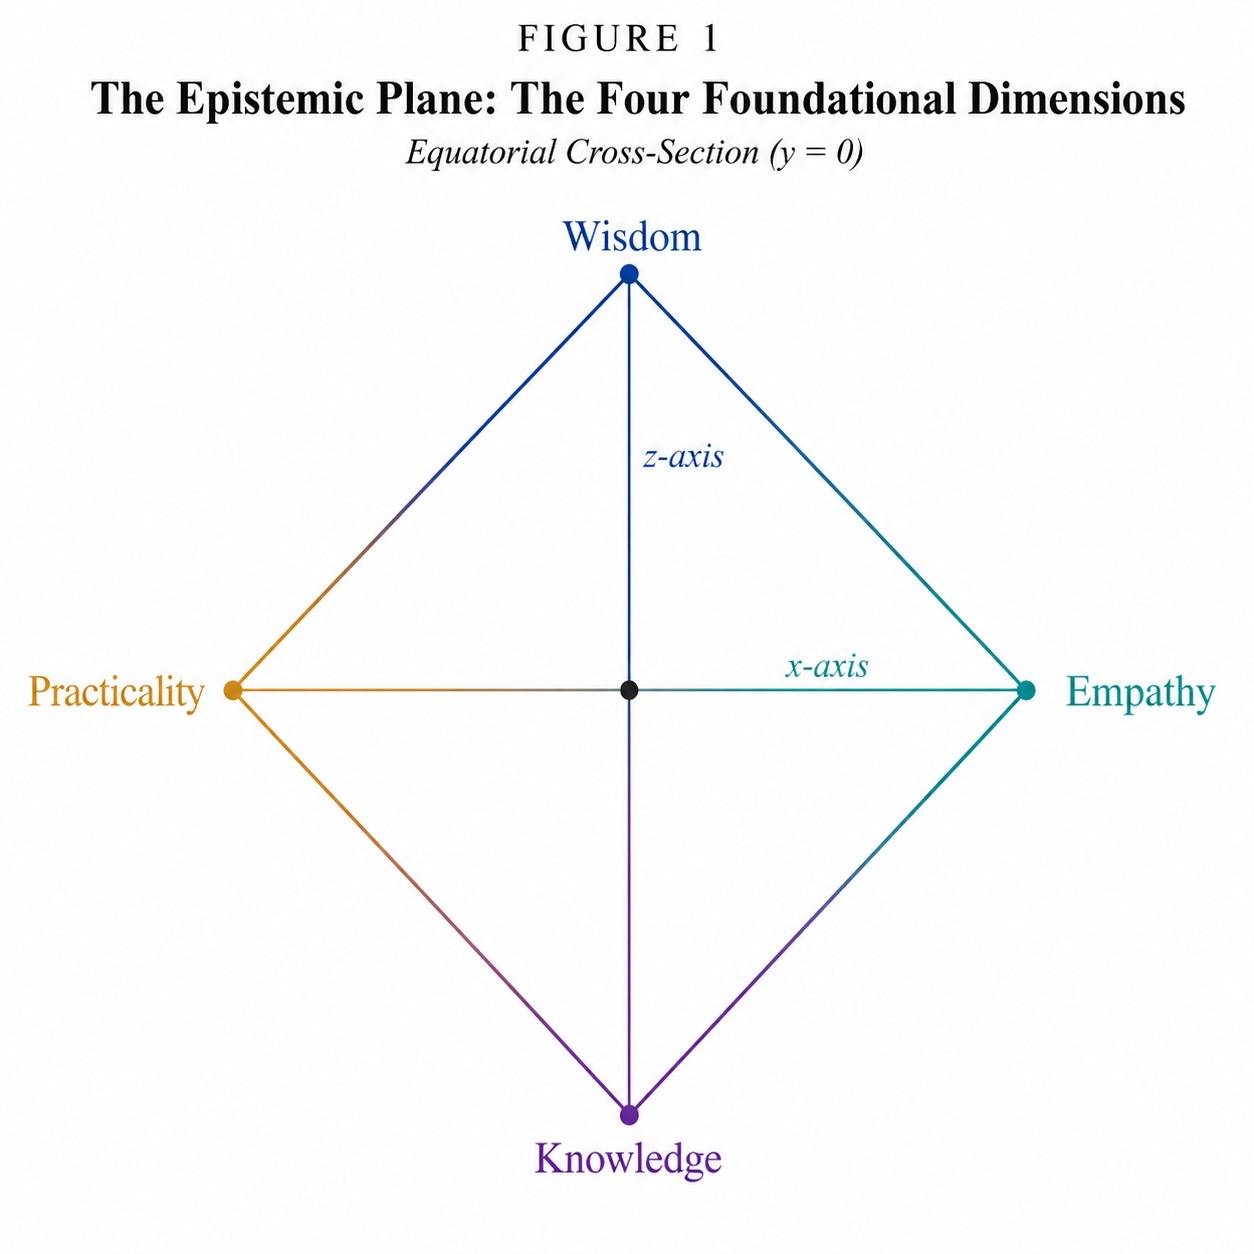
\includegraphics[width=0.92\linewidth]{figure1_epistemic_plane.jpeg}
\end{center}

\begin{center}
    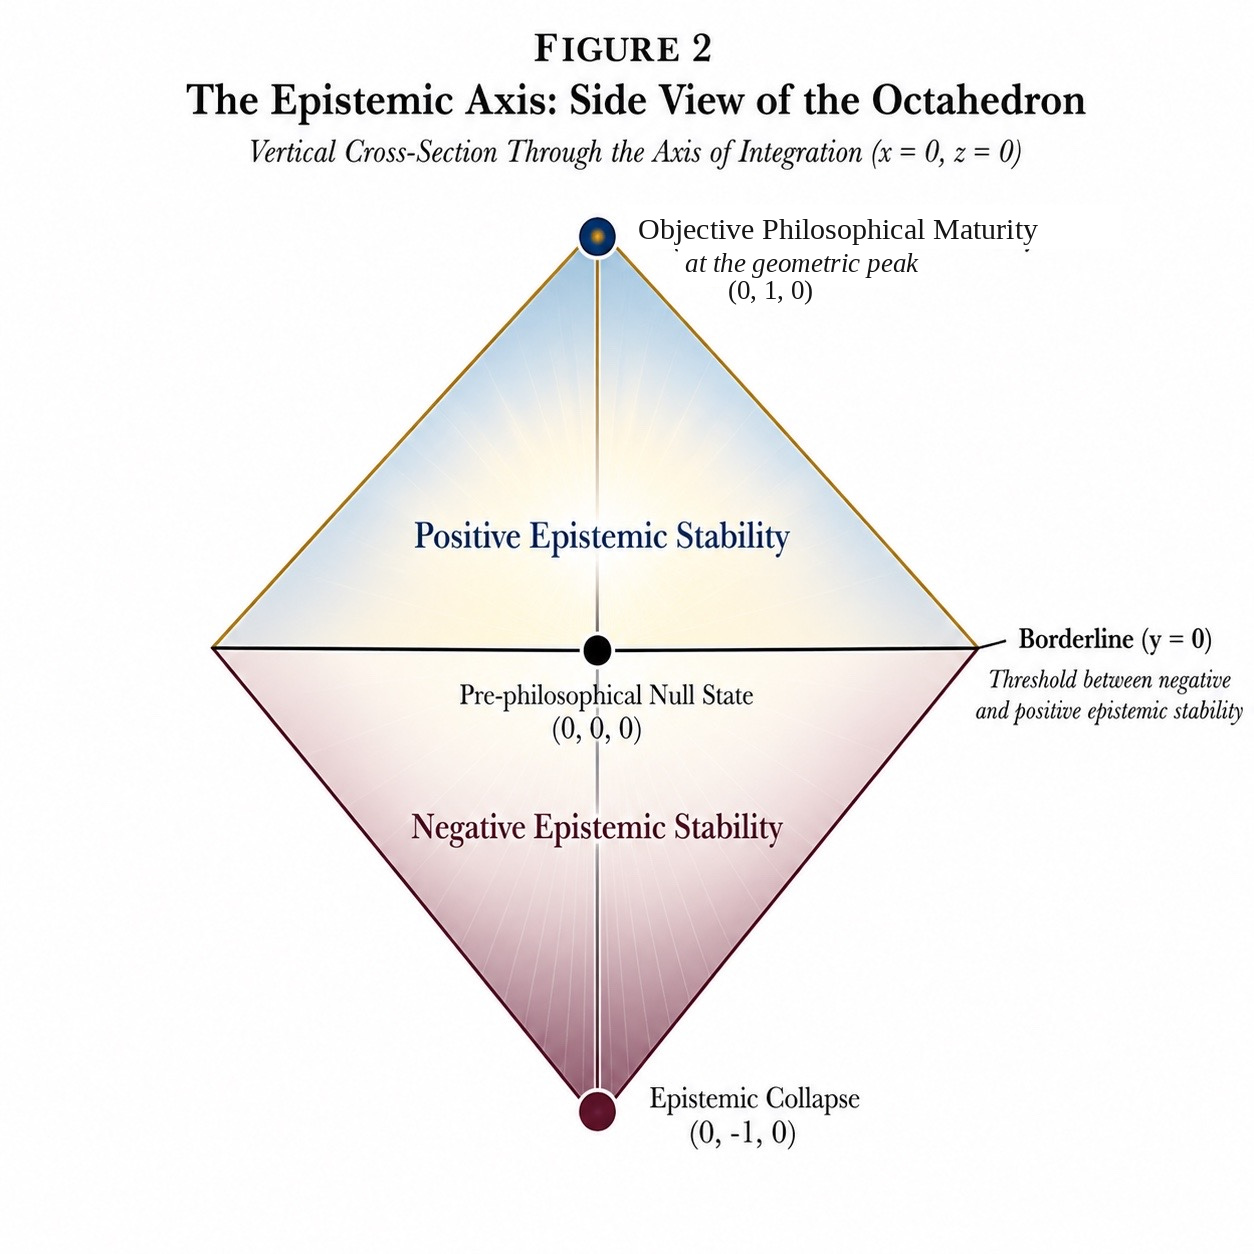
\includegraphics[width=0.92\linewidth]{figure2_epistemic_axis.jpeg}
\end{center}

\section{Why an Octahedron}

The octahedron is the correct geometry for this model because it combines opposed dimensions with a single surface constraint. The geometry matters because the model is not merely naming traits. It is representing how mature judgment relates concern, constraint, information, judgment, and epistemic stability within one structure.

First, the horizontal dimensions are bipolar tensions. Empathy and practicality are not merely separate virtues; they can compete for emphasis when judgment is immature, partial, or context-blind. Wisdom and knowledge behave similarly. Knowledge without wisdom may become technical narrowness. Wisdom without sufficient knowledge may become vague intuition. This does not mean mature wisdom can exist with no knowledge. It means a worldview-state, stance, text, or system may be oriented toward context, limits, interpretation, and application while little or no informational grounding is actively contributing to that referent. Empathy without practicality may become reality-detached sentiment. Practicality without empathy may become functional coldness. The octahedron represents these tensions without reducing them to a flat spectrum.

The surface constraint should not be read as claiming that empathy, practicality, wisdom, and knowledge are finite substances that must be traded away against one another. It represents philosophical orientation within the referent being plotted. Lateral coordinate displacement represents structural orientation within the declared referent. Visible contextual emphasis is a separate evidential object and does not by itself establish structural displacement. Where lateral displacement is present, its meaning may range from correctable asymmetry to entrenched distortion depending on epistemic stability. At the top vertex, the disappearance of lateral displacement does not mean the disappearance of the horizontal dimensions. It means their integration under maximal positive epistemic stability.

Second, the octahedron gives privileged status to vertical culmination. The top and bottom are vertices, not ordinary regions. This matches the semantics of the model. Mature integration and epistemic collapse are not merely two more positions among many. They are limiting states. The upper vertex is the complete positive limit of reality-governed integration. The lower vertex is the complete negative limit: the collapse of reality-governed integration itself.

Third, the surface constraint prevents interpretive looseness. A worldview position must be placed relative to the necessary functions of worldview formation. Lateral displacement, vertical stability, and distance from the peak are all part of the same structure. The graph therefore represents not only category but orientation.

Fourth, the model preserves the origin without turning the interior into plotted space. This solves a basic structural problem. The model needs a way to reference pre-worldview states without confusing them with epistemic failure inside a formed worldview. Reserving the origin for the null state achieves this without weakening the surface geometry.

\section{Definitions}

\begin{definition}[Worldview]
A worldview is a formed organization of reasoning that takes a structured stance toward reality through concern for affected persons, practical constraint, informational grasp, contextual discernment, and epistemic stability. It may be explicit or tacit, currently expressed or dormant, stable or unstable. Mental organization preceding this level of formation is pre-worldview rather than an inactive worldview.
\end{definition}

\begin{definition}[Epistemic Stability]
Epistemic stability is the degree to which a worldview remains coherent, reality-tracking, self-corrective, and resistant to delusion under internal reflection and external pressure.
\end{definition}

\begin{definition}[Wisdom]
Wisdom, as used in this model, is contextual discernment. It is the capacity to interpret knowledge, weigh context, recognize limits, preserve proportion, anticipate consequences, and govern application. It is not moral purity, compassion, benevolence, or the whole condition of philosophical maturity. It is the judgmental counterpart to knowledge, not the peak itself. Knowledge feeds wisdom, and wisdom governs knowledge; the graph separates them only to represent how active reasoning may over-orient toward one function when it has not yet integrated both.
\end{definition}

\begin{definition}[Objective Philosophical Maturity]
Objective philosophical maturity is the state represented at the top vertex of the Epistemic Octahedron, also called the geometric peak or the upper vertex in coordinate terms. It denotes mature integration of empathy, practicality, wisdom, and knowledge under maximal positive epistemic stability.
\end{definition}

\begin{definition}[Pre-Philosophical Null State]
The pre-philosophical null state is represented by the coordinate origin $(0,0,0)$. It denotes the absence of a worldview: mental organization has not yet formed a structured stance toward reality of the kind represented on the octahedral surface. Infancy is one example, but the concept is broader than age.
\end{definition}

\begin{definition}[Epistemic Collapse]
Epistemic collapse is represented by the lower vertex $(0,-1,0)$. It denotes maximal negative epistemic stability: the limiting state in which reality-governed integration has collapsed and the worldview no longer remains answerable to correction.
\end{definition}

\begin{definition}[Worldview Formation Boundary]
The worldview formation boundary separates pre-worldview mental organization from a worldview. Once reasoning forms a structured stance toward reality through concern, constraint, information, interpretation, and epistemic stability, it is a worldview and has a position on the octahedral surface. States preceding this boundary may be referenced by the model through the null origin, but they are not worldviews.
\end{definition}

\begin{definition}[Truth-Relation]
Truth-relation is the way a worldview relates to reality through speech, silence, disclosure, concealment, framing, evidence, interpretation, and correction.
\end{definition}

\begin{definition}[Truth-Action]
A truth-action is any communicative act that shapes another person's access to reality, including disclosure, refusal, silence, concealment, framing, redirection, and false communication.
\end{definition}

\begin{definition}[Lie]
A lie, in the strict descriptive sense, is an intentional falsehood communicated so that another person will believe what the speaker takes to be false. Its mature or immature status is determined by its relation to integrated accountability.
\end{definition}

\begin{definition}[Accountability]
Accountability is the active relation by which a worldview remains answerable to reality, affected persons, consequences, information, context, and correction after a truth-action or failure.
\end{definition}

\begin{definition}[Moral Judgment]
Moral judgment is worldview judgment applied to normative questions: what ought to be done, protected, condemned, permitted, owed, or valued. In this model, moral judgment is not an isolated faculty separate from worldview formation. It is a domain in which the structure of worldview formation becomes normatively expressed.
\end{definition}

\begin{definition}[Source-Mediated Learning]
Source-mediated learning is the acquisition or revision of a belief through information supplied by another epistemic agent, including a person, text, institution, tradition, system, or recorded observation. The term identifies the route by which information enters the recipient; it does not by itself determine whether the resulting belief is mature, unstable, true, or false.
\end{definition}

\begin{definition}[Receptive Learning]
Receptive learning is source-mediated learning in which the recipient allows received information to affect a working model while retaining authorship over its interpretation, confidence, application, and correction. It may be passive at the point of acquisition while remaining active and reality-governed at the point of integration.
\end{definition}

\begin{definition}[Epistemic Source Weight]
Epistemic source weight is the defeasible contribution that a source's testimony makes to rational confidence relative to the declared referent. It depends on evidence concerning the source's reality-contact, competence, access, transparency, incentives, communicative purpose, and correction history. Source weight modifies confidence; it does not replace reality or convert testimony into proof.
\end{definition}

\begin{definition}[Epistemic Continuity]
Epistemic continuity is the principle that a source's previously demonstrated reality-contact and correction-responsiveness remain relevant to later communications. Continuity is defeasible and domain-sensitive: it preserves earned epistemic standing without granting permanent authority, whole-person infallibility, or immunity from renewed evaluation.
\end{definition}

\begin{definition}[Verification Threshold]
A verification threshold is the degree of independent examination proportionately required before a received claim should govern belief or action. The threshold rises with stakes, novelty, irreversibility, contradiction, weak source access, unreliable correction history, and incentives for deception; it may remain lower when the claim is low-stakes, provisional, reversible, and supported by a source with established domain-relevant stability.
\end{definition}

\section{Referent of a Plot}

The Epistemic Octahedron defines the structure of philosophical orientation. A plotted point must therefore have a referent: a whole worldview, a current philosophical state, a stance, a fragment of reasoning, a written text, an institutional orientation, a system, or another philosophically meaningful unit of analysis. The geometry and semantics do not change across these uses. What changes is the evidential breadth of the claim being made.

A point based on a narrow fragment should not be interpreted as a certification of an entire enduring worldview. Likewise, a thin or underdetermined expression should not be mistaken for mature integration merely because it contains no explicit defect. The top vertex represents integration relative to the referent being assessed. Stronger claims about whole-worldview maturity require evidence broad enough to support that referent.

This distinction preserves the openness of the model without weakening its objectivity. A perfect instrument that could capture an entire worldview would still use the same graph. A narrower instrument that evaluates a fragment of reasoning would also use the same graph, but its result would be limited to that fragment.

The coordinates should therefore be read as orientation-values. For example, a pure knowledge-side position does not mean a literal human being with no other mental content. It means that, within the assessed referent, informational grasp is doing the organizing work while contextual discernment, person-directed concern, and functional constraint are not materially contributing. A book, database, argument, expert performance, bureaucratic procedure, algorithm, or individual stance can occupy such limiting regions when the referent is defined appropriately.

\subsection{Expression, Underlying Reasoning, and Communicative Purpose}

A plot must distinguish the reasoning being assessed from the amount of that reasoning made explicit in a particular utterance. Human communication is routinely compressed. A person may state a conclusion, show an illustration, mention an example, remain silent about intermediate steps, or rely on shared context without presenting the entire evidential history that produced the judgment. The visible expression is evidence about the underlying reasoning, but it is not automatically identical to that reasoning.

This distinction is structurally necessary. Inferring that a person performed no due diligence merely because the person did not disclose a full argument confuses \emph{undisclosed reasoning} with \emph{absent reasoning}. The inference becomes valid only when the referent is explicitly the presented argument, or when the communicative act claimed to provide sufficient proof, or when broader evidence shows that the omitted reasoning did not exist or could not withstand correction. A casual report of belief, an illustrative example, and an attempt at persuasion are different truth-actions because they place different demands on evidence presentation, listener uptake, and accountability.

Communicative purpose therefore belongs to contextual discernment. A listener should ask what the speaker was doing: reporting an impression, inviting discussion, supplying an example, requesting trust, asserting certainty, or attempting to transfer belief. The same sentence can have different epistemic force across those purposes. Mature interpretation does not excuse deception or reckless overstatement, but it also does not manufacture a stronger claim and then punish the speaker for failing to defend that manufactured version.

Conversational compression is compatible with peak reasoning when the omitted qualifications remain genuinely integrated in the underlying judgment and the compression is proportionate to the setting. Precision is required where stakes, foreseeable misunderstanding, authority, or imposed consequences make it materially relevant. Where no such pressure exists, mature reasoning may communicate economically without converting every ordinary statement into a formal proof.

The recipient side requires a corresponding distinction. Expression--reasoning non-identity does not require the listener to accept an unseen basis as sufficient. It requires the listener to avoid treating nondisclosure as proof of nonexistence. A recipient may withhold adoption of the conclusion, assign it limited weight, ask for clarification, or raise the verification threshold without claiming that the source performed no reasoning. Where the source has a relevant epistemic history, that history may rationally affect the provisional weight of a compressed judgment. Where no such history exists, uncertainty can be preserved without manufacturing either confidence or dismissal.

\begin{proposition}[Expression--Reasoning Non-Identity]
The evidential content of an utterance and the structure of the reasoning that produced it are related but non-identical referents. Failure to present a complete argument establishes only that the complete argument was not presented. It does not, without further evidence, establish that the underlying judgment was formed without due diligence.
\end{proposition}

\begin{proposition}[Purpose-Sensitive Evidential Demand]
The amount and form of evidence maturely required in communication depend on the truth-action being performed. Reporting a revisable impression, illustrating a topic, inviting inquiry, and attempting persuasion impose different evidential burdens. Epistemic evaluation that ignores this difference mislocates the referent and can mistake conversational economy for instability.
\end{proposition}

\begin{proposition}[Disclosure--Basis Non-Identity]
The evidence disclosed in one communicative act does not necessarily exhaust the source's basis of judgment. A recipient may rationally remain unconvinced while still assigning the testimony provisional weight according to broader evidence about the source, domain, and referent. Limited disclosure establishes limited presentation, not by itself absent due diligence.
\end{proposition}

\section{Null Origin and Integrated Balance}

The most important distinction in the model is the distinction between two forms of non-asymmetry.

At the coordinate origin, the horizontal dimensions are not in tension because no worldview has yet formed. This is not maturity and not pathology. It is pre-philosophical absence.

At the top vertex, the horizontal dimensions are also no longer in unresolved lateral conflict, but for the opposite reason. They have been encountered, tested, and integrated under positive epistemic stability. This is mature balance.

The null origin and the peak may both lack lateral displacement, but they are not equivalent. One is absence before development. The other is integration after development. Confusing them would make maturity indistinguishable from pre-worldview absence.

\begin{proposition}
The pre-philosophical null state at the origin and the mature integrated state at the top vertex are structurally non-equivalent. The former is non-asymmetry by absence of worldview formation. The latter is non-asymmetry by reflective integration.
\end{proposition}

This proposition allows the model to distinguish absence, failure, and maturity without contradiction. It also prevents the lower vertex from being misread as the beginning of development. The lower vertex is not infancy, ignorance, or neutrality. It is epistemic collapse.

\section{Interpretation of the Lower Half}

The lower half of the Epistemic Octahedron is structured negative space. It should not be treated as a single undifferentiated category. It contains multiple forms of non-mature worldview organization, including:

\begin{itemize}
    \item distorted reality-tracking,
    \item immaturity,
    \item delusion,
    \item false certainty,
    \item refusal of correction,
    \item negative epistemic stability.
\end{itemize}

These conditions are related because each involves failure of mature epistemic organization, but they are not identical. The model allows them to appear in different lower-half regions depending on lateral emphasis.

A lower-half position displaced toward knowledge may indicate technical confidence without wisdom. A lower-half position displaced toward wisdom may indicate false profundity, over-interpretation, or pseudo-discernment without adequate reality-contact. A lower-half position displaced toward empathy may indicate concern severed from reality-contact. A lower-half position displaced toward practicality may indicate functional calculation without reflective integration. These are not the same failure. The lower half therefore represents a structured field of worldview-level instability rather than a general label for ``bad'' reasoning.

Passive ignorance does not by itself imply the lower vertex. A person may be uninformed, hesitant, or undeveloped without being epistemically collapsed. Deep descent in the model is reserved for stronger failures: entrenched distortion, self-sealing belief, refusal of correction, false certainty, or reality-detachment.

This distinction is necessary because any serious model of maturity must separate ignorance, underdevelopment, one-sidedness, delusion, and collapse. Treating them as the same would destroy the model's diagnostic value.

The lower vertex is the collapse of reality-governed integration itself. At this limit, the four horizontal dimensions no longer correct one another. Empathy, practicality, wisdom, and knowledge remain structurally present, but they have been absorbed into distortion, rationalization, self-protection, or delusional preservation. The lower vertex is therefore the exact negative limit of the upper vertex: where the upper vertex represents total reality-governed integration, epistemic collapse is total failure of reality-governed integration.

\section{Why the Null State Is Not the Lower Vertex}

Because the origin represents the pre-philosophical null state, the model does not classify pre-worldview states as negative epistemic stability. Infancy is a clear reference case of pre-worldview absence rather than epistemic collapse.

Development therefore does not require literal passage through the lower vertex or every lower-half region. A worldview may emerge near the equator, in the lower half, or in the lower positive range depending on its structure. The graph distinguishes logical reference points from actual developmental trajectories.

This is one of the model's key advantages. It avoids the mistake of treating early absence as pathology while still preserving a sharp concept of epistemic failure within a formed worldview.

\section{The Top Vertex: Full Integration at the Geometric Peak and Objective Philosophical Maturity}

Within this framework, the top vertex names the geometric peak of the octahedron. Semantically, that peak is the point at which positive epistemic stability reaches its maximal form and the constitutive tensions of the model have been fully integrated. The result at that geometric peak is objective philosophical maturity: the mature relation of empathy, practicality, wisdom, and knowledge under coherence, reality-contact, self-correction, and resistance to delusion.

A mature person may still emphasize one dimension in a given context. Practicality may dominate during a crisis. Empathy may dominate in caregiving. Knowledge may dominate in technical inquiry. Wisdom may dominate when context, proportion, limits, and application matter most. Such emphasis remains mature when it is governed by the integrated structure rather than produced by a neglected dimension.

This gives the top vertex an important form of integrated flexibility. When two mature agents confront an unprecedented crisis, they may emphasize different dimensions because the crisis itself contains multiple valid pressures that have not yet been fully reconciled. One agent may lead with empathy because immediate suffering has become morally urgent. Another may lead with practicality because long-term survival has become structurally decisive. The maturity of the disagreement is measured by the continued answerability of both judgments to the full structure: affected persons, practical constraint, information, context, consequences, and correction.

Peak-level disagreement therefore becomes a higher-order form of inquiry. Once ordinary noise is removed, including ego-defense, ideological capture, missing information, sentimental evasion, cold calculation, and refusal of correction, the remaining disagreement marks a genuine pressure inside reality. The emphasized dimension becomes worth serious consideration precisely because the other dimensions have not been abandoned. Such disagreement has less friction than ordinary subjectivity because it remains corrigible, transparent, and reality-bound. It does not degrade discourse; it presses understanding farther into the unresolved structure of the crisis.

The same structure also changes instinctive response. At lower maturity, reflex often means blind impulse: the agent reacts before the relevant dimensions have been integrated. At the top vertex, reflex can become trained immediacy. The first movement of judgment may become more objectively reliable because the structure beneath it has already integrated the dimensions that immature reflex usually skips. Mature immediacy is therefore not mere speed. It is the fast expression of a reality-governed structure.

Maturity in this model therefore means:

\begin{itemize}
    \item the person has encountered the four dimensions rather than remaining blind to them,
    \item the person understands what each dimension contributes,
    \item the person is not trapped in one-axis reasoning,
    \item the person can shift emphasis without losing orientation,
    \item the person's worldview remains reality-tracking and self-corrective.
\end{itemize}

The peak is a claim about structural completion at the top vertex. A person at or near the peak may still acquire new information, revise conclusions, change applications, and adapt to new circumstances. What has matured is the structure by which judgment remains integrated and reality-bound, not the total amount of knowledge possessed at a given moment.

\subsection{Peak Inclusion and the Burden of Displacement}

The positive vertical conditions are nested within mature integration. Reality-intactness names the capacity for facts, consequences, constraints, and correction to discipline a worldview. Self-correction names the stronger capacity to revise the worldview under pressure. Philosophical maturity contains both capacities and integrates them with empathy, practicality, wisdom, and knowledge. A top-vertex referent is therefore also reality-intact and self-corrective; the lower positive labels identify partial or less completely integrated expressions of capacities that remain present at the peak.

The vertical gates should consequently not be read as mutually exclusive floors through which a referent passes and then leaves behind. They are semantic cross-sections of increasingly complete reality-governed organization. A single act of accepting correction may evidence self-correction without securing the whole referent at the self-corrective level. Conversely, a peak-level fragment does not cease to contain self-correction merely because its coordinate is $y=1$ rather than $y=\frac{2}{3}$.

For a properly bounded referent, exact peak is warranted when every materially relevant pressure available within that referent remains governing: affected persons, practical constraint, informational grounding, contextual discernment, consequences, and correction. A lower placement requires identifying a real displacement condition, not merely pointing to fallibility, incomplete knowledge, compressed expression, or the abstract possibility of error. Those features are compatible with peak because peak concerns the mature structure by which the referent remains answerable to reality, not omniscience or exhaustive verbalization.

\begin{proposition}[Cumulative Positive Integration]
For any fixed referent, the top vertex includes the positive capacities named by the lower positive gate labels in fully integrated form. Reality-intactness and self-correction are constitutive functions of philosophical maturity, not regions excluded by it.
\end{proposition}

\begin{proposition}[Relevant-Pressure Criterion]
A referent departs from the top vertex only when at least one materially relevant pressure fails to govern the judgment because it is absent, suppressed, distorted, or insulated from correction. Mere uncertainty, limited information, contextual emphasis, concise expression, or the possibility of future revision does not by itself establish departure from peak.
\end{proposition}

When applied to morality, this means that the best moral judgment does not begin as an unresolved leaning toward one horizontal pole. It begins from integrated stability and then emphasizes whatever the situation requires. Context-sensitive emphasis is not the same as imbalance. Imbalance occurs when one function dominates because the others are absent, suppressed, or distorted. Mature emphasis occurs when one function leads in action while remaining accountable to the whole integrated structure.

\section{Source-Mediated Learning under Epistemic Stability}

The Epistemic Octahedron does not apply only after an isolated individual has already formed a belief. Its semantic structure also governs how worldviews receive information from other worldviews. Once concern, constraint, information, interpretation, and epistemic stability are recognized as objective structural functions, a psychological consequence follows: mature learning cannot require that every person independently reconstruct every item of knowledge from direct contact with reality. Human knowledge is socially distributed, yet the recipient remains answerable to reality.

This section develops that consequence. The central distinction is between the route by which information is acquired and the structure by which it is integrated. Information may arrive passively through testimony, instruction, observation of another person's judgment, inherited practice, or institutional transmission. The resulting worldview-state may still occupy the positive half of the octahedron when the recipient weighs the information proportionately, preserves uncertainty, matches verification to consequence, and remains open to correction. Passive receipt is therefore compatible with active epistemic authorship.

\subsection{The Social Dependence of Human Knowledge}

No human being can personally inspect the full evidential basis of ordinary life. A person learns language before independently verifying linguistic convention, receives historical knowledge without witnessing the events, depends on specialized competence outside personal training, and uses social testimony to navigate places, people, risks, customs, and institutions. Even direct observation depends on inherited concepts, measurement systems, and methods learned from others.

This dependence creates a permanent psychological problem. A learner must receive information from sources that can be mistaken, deceptive, status-driven, ideologically captured, technically competent but context-blind, morally sincere but factually weak, or reliable only inside a narrow domain. The impossibility of universal verification does not remove these risks. It requires a mature structure for managing them.

The octahedron rejects two symmetrical reductions. Blind acceptance allows the source to replace reality. Universal suspicion treats the absence of firsthand verification as sufficient reason to reset every claim to zero. The first abandons authorship to authority, affiliation, confidence, or familiarity. The second abandons practical and social reality by demanding an impossible independence from distributed knowledge. Mature reception lies in neither extreme. It gives testimony graded, corrigible, referent-sensitive weight.

\subsection{Acquisition and Integration Are Different Referents}

The route of acquisition does not determine the maturity of the belief. The same statement may be received by two people and integrated differently. One person may absorb it as unquestionable because a parent, expert, institution, friend, or admired figure said it. Another may preserve it as a provisional input, compare it with other information, notice the source's limits, and revise it when contrary evidence appears. Both acquired the information socially. Their epistemic structures differ.

This establishes an acquisition--integration distinction parallel to expression--reasoning non-identity. The first distinction prevents the recipient from mistaking socially received knowledge for unowned thought. The second prevents the evaluator from mistaking incomplete expression for incomplete reasoning. Together they show that mature cognition cannot be located solely by asking where a statement came from or how much of its basis was displayed. The relevant question is how the full referent remains governed by reality.

Receptive learning can therefore be passive in a limited and non-pathological sense: the recipient did not generate the original observation, argument, or expertise. The recipient remains active in the structurally decisive sense by governing confidence, interpretation, application, and correction. Authorship concerns the organization of received material, not the impossible requirement that all material originate within the self.

\begin{proposition}[Acquisition--Integration Non-Identity]
The external receipt of information does not determine the epistemic maturity of the resulting belief. Source-mediated acquisition is compatible with any vertical region of the octahedron; its location depends on how the recipient weighs, interprets, applies, and corrects the information within the declared referent.
\end{proposition}

\subsection{Source, Message, Recipient, and Reality}

Source-mediated learning contains at least four distinct epistemic objects:

\begin{enumerate}[label=\arabic*.]
    \item the source's access to reality and underlying judgment;
    \item the message or expression actually transmitted;
    \item the recipient's interpretation, confidence, and use of that message;
    \item the reality to which both source and recipient remain answerable.
\end{enumerate}

These objects may diverge. A mature source may communicate poorly. An unstable source may accidentally report something true. A compressed message may rest on broad reasoning, while an elaborate message may conceal a weak basis. A mature recipient may extract limited useful information from a distorted source, while an unstable recipient may convert careful testimony into dogma, panic, resentment, or identity-defense. The truth of the claim cannot be reduced to the source's status, and the source's epistemic standing cannot be reduced to the truth-value of one claim.

\begin{center}
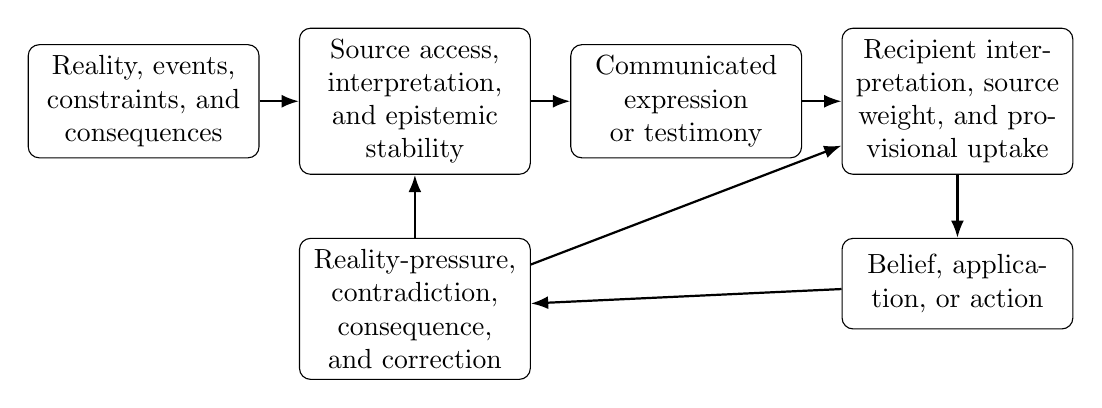
\begin{tikzpicture}[
  node distance=8mm and 5mm,
  box/.style={draw, rounded corners, align=center, text width=2.65cm, minimum height=1.15cm, inner sep=4pt},
  arrow/.style={-{Latex[length=2.2mm]}, thick}
]
\node[box] (reality) {Reality, events, constraints, and consequences};
\node[box, right=of reality] (source) {Source access, interpretation, and epistemic stability};
\node[box, right=of source] (message) {Communicated expression or testimony};
\node[box, right=of message] (recipient) {Recipient interpretation, source weight, and provisional uptake};
\node[box, below=of recipient] (action) {Belief, application, or action};
\node[box, below=of source] (correction) {Reality-pressure, contradiction, consequence, and correction};
\draw[arrow] (reality) -- (source);
\draw[arrow] (source) -- (message);
\draw[arrow] (message) -- (recipient);
\draw[arrow] (recipient) -- (action);
\draw[arrow] (action) -- (correction);
\draw[arrow] (correction) -- (source);
\draw[arrow] (correction) -- (recipient);
\end{tikzpicture}
\par\smallskip
{\small\textbf{Figure 3.} Source-mediated learning under epistemic stability. Testimony passes through source interpretation and recipient uptake while both remain answerable to correction.}
\end{center}

The figure shows why neither personal trust nor claim-testing can operate alone. A source history can rationally affect initial confidence, but reality retains final authority. A message can be considered without being adopted, and a belief can be acted upon provisionally without being protected from later correction.

\begin{proposition}[Source--Truth Non-Identity]
Source reliability and claim truth are related but distinct. A reliable source can be mistaken, and an unreliable source can communicate truth. Source weight may rationally alter confidence, but no source position, credential, relationship, status, or reputation replaces the reality to which the claim remains answerable.
\end{proposition}

\subsection{Epistemic Source Weight and Continuity}

Mature source evaluation is graded rather than binary. Testimony may slightly raise confidence, strongly raise confidence, justify provisional acceptance, justify immediate low-risk action, or carry almost no weight. The degree depends on the referent. A person's demonstrated stability in technical work does not automatically transfer to moral character, political judgment, family conflict, or another specialized domain. Whole-person admiration cannot substitute for domain-relevant access and competence.

At the same time, mature learning does not reset a known source to epistemic zero during every exchange. Prior reality-contact, careful distinction, willingness to admit uncertainty, successful prediction, correction under pressure, and transparent acknowledgment of error are themselves evidence. Epistemic continuity preserves that evidence. A compressed statement from a repeatedly careful source can rationally receive more provisional weight than the same statement from an unknown or repeatedly deceptive source.

Continuity remains defeasible. New contradictions, hidden incentives, domain transfer, repeated overconfidence, manipulation, or resistance to correction may lower the source's weight. One error need not erase a long history, while one success need not establish enduring reliability. The mature recipient updates both the proposition and the model of the source.

This structure answers the difficulty posed by malintent, bad faith, status manipulation, appeal to authority, and concealed incentives. These possibilities do not force universal distrust. They are pressures to be weighed. Their relevance rises when the source benefits from belief, conceals access, demands submission, blocks independent checking, changes standards under pressure, or uses status as a substitute for explanation. Their relevance falls when the source openly marks uncertainty, separates observation from interpretation, accepts correction, and remains within demonstrated competence.

\begin{proposition}[Epistemic Continuity]
Previously demonstrated source stability supplies defeasible, domain-sensitive evidence for later source weighting. Rational evaluation need not begin from zero in every exchange, but accumulated trust never becomes permanent authority or immunity from contradiction.
\end{proposition}

\subsection{Proportional Verification}

Verification is necessary, but its mature form is proportional. The demand for independent examination should rise with the cost of error. A medical intervention, criminal accusation, irreversible financial decision, public policy, or claim carrying severe consequences requires a higher threshold than a casual impression, reversible preference, low-stakes observation, or information offered only for consideration.

The verification threshold also rises when the claim is novel, conflicts with strong existing evidence, depends on inaccessible private knowledge, comes from a source with weak domain competence, or appears under incentives for deception. It may remain lower when the source has direct access, established domain-relevant stability, a transparent basis, no demand for compulsory uptake, and a history of correction.

Universal verification is not maximal maturity. It can become a knowledge-side distortion when the recipient treats visible proof as the only rational basis for provisional uptake, ignores contextual source evidence, and imposes the cost of a formal argument on every low-stakes communication. The opposite distortion accepts testimony because verification is inconvenient. Peak judgment integrates both: it spends attention where reality and consequence require it.

A grain of salt is therefore not mere vagueness. Structurally, it means that the information enters the recipient's working model with limited confidence, restricted scope, and preserved correction conditions. The claim may guide attention without governing action, increase plausibility without producing belief, or justify temporary action without being treated as final truth.

\begin{proposition}[Proportional Verification]
Mature inquiry matches independent verification to stakes, reversibility, contradiction, source access, source stability, and foreseeable consequence. Universal credulity and universal firsthand verification both fail to integrate the full structure of learning.
\end{proposition}

\subsection{The Horizontal Dimensions in Source-Mediated Learning}

The four horizontal dimensions explain why source evaluation cannot be reduced to fact-checking or trust.

\begin{itemize}
    \item \textbf{Knowledge} tracks what the source knows, what was observed, what evidence was disclosed, and what remains unknown.
    \item \textbf{Wisdom} interprets domain, motive, limits, context, confidence, indirect evidence, communicative purpose, and the difference between a revisable impression and an attempted proof.
    \item \textbf{Practicality} recognizes finite time, unequal access, division of expertise, reversible action, and the real cost of verifying every claim from the beginning.
    \item \textbf{Empathy} treats source and recipient as persons whose trust, vulnerability, good faith, manipulation, misunderstanding, and consequences matter, without allowing concern or affiliation to replace truth.
\end{itemize}

No single dimension can govern mature source learning alone. Knowledge without wisdom may demand visible evidence while misreading purpose, scope, or source history. Wisdom without knowledge may overread motives and hidden meanings. Empathy without practicality may trust from attachment or moral sympathy. Practicality without empathy may use sources instrumentally while ignoring deception, dignity, or harm. The vertical axis determines whether these pressures remain integrated, corrigible, and reality-governed.

\begin{center}
\begin{tabular}{>{\raggedright\arraybackslash}p{4.1cm} >{\raggedright\arraybackslash}p{9.1cm}}
\toprule
Structural distortion & Expression in source-mediated learning \\
\midrule
Empathy-side distortion & Belief from attachment, sympathy, shared identity, vulnerability, fear of offending, or desire to preserve belonging. \\
Practicality-side distortion & Acceptance or rejection based only on usefulness, efficiency, institutional convenience, social order, or immediate results. \\
Wisdom-side distortion & Overreading motives, symbolism, subtext, hidden coordination, or personal intuition without enough informational grounding. \\
Knowledge-side distortion & Credential worship, isolated fact-checking without context, compulsive proof demands, or treating disclosed evidence as the source's entire basis. \\
Negative epistemic instability & Filtering sources through identity-protection, resentment, fear, status, ideology, dependency, or correction-resistant distrust. \\
Peak integration & Graded source weight, domain discipline, proportional verification, retained authorship, humane interpretation, practical efficiency, and continuing correction. \\
\bottomrule
\end{tabular}
\end{center}

\subsection{Positive Epistemic Gates in Receptive Learning}

Source-mediated learning can occur throughout the positive half. The positive gates do not require the learner to originate all information, and they do not convert increased maturity into increased suspicion.

At \emph{Reality-Intact}, the recipient distinguishes testimony from reality. A claim may be considered or provisionally accepted, but facts, consequences, contradiction, and direct evidence can still discipline it. The source has influence without becoming an untouchable authority.

At \emph{Self-Corrective}, the recipient can revise not only the received belief but also the confidence assigned to the source. Discovery of error may narrow the source's domain, expose an incentive, distinguish accidental mistake from deception, or strengthen trust when the source corrects itself openly.

At the top vertex, source, message, domain, affected persons, practical limits, uncertainty, consequences, and correction are integrated. Peak learning does not require maximal distrust. It includes the capacity to trust proportionately, learn efficiently, and increase verification when a materially relevant pressure demands it.

The negative half contains structurally different failures. A correction-locked recipient may preserve a source because affiliation or identity depends on it, or preserve distrust because accepting testimony would feel like submission. A reality-fractured recipient may alternate between credulity and suspicion according to emotion, status, or group pressure. At collapse, source evaluation no longer tracks reality; information is sorted only by whether it protects the defended worldview.

\begin{proposition}[Correction-Preserving Uptake]
Source-mediated learning remains positively stable when the recipient can revise the received belief, its confidence, its application, and the source's future weight under reality-pressure. The source may guide learning without acquiring authority over correction.
\end{proposition}

\subsection{Psychological and Educational Consequence}

The model therefore identifies a capacity that ordinary appeals to ``critical thinking'' often leave unspecified: the ability to receive socially transmitted knowledge under retained authorship. Psychological maturity does not eliminate dependence on other minds. It organizes that dependence so that trust, skepticism, uncertainty, and correction remain proportionate.

A learner who has not developed this structure may confuse consideration with submission, uncertainty with weakness, trust with gullibility, skepticism with intelligence, or credentials with truth. Education can then produce either obedient repetition or compulsive challenge while failing to teach source weighting. The octahedron supplies the missing objective structure: learners should be trained to locate the referent, distinguish source from message, assess access and competence, preserve graded confidence, match verification to stakes, and update both belief and source weight under correction.

This is a psychological implication of the semantic model itself rather than an external educational preference. A formed worldview necessarily handles information and interpretation under practical and interpersonal conditions. Because much information arrives through other agents, the mature integration of the horizontal dimensions under positive epistemic stability necessarily includes mature receptive learning.

\section{Formal Semantic Kernel of the Epistemic Octahedron}

The preceding sections define the ontology and interpretation of the Epistemic Octahedron in prose. The present section states the same structure in compact mathematical form. The notation formalizes the geometry and semantic relations of the model; it does not yet prescribe a psychometric scoring procedure.

\subsection{Octahedral State-Space and Surface Projection}

Let
\[
\mathbb O
:=
\left\{
p\in\mathbb R^3:
\|p\|_1\leq1
\right\}
\]
denote the complete octahedral solid, where
\[
\|p\|_1=|x|+|y|+|z|.
\]

Its boundary is
\[
\partial\mathbb O
:=
\left\{
p\in\mathbb R^3:
\|p\|_1=1
\right\}.
\]

Only the boundary $\partial\mathbb O$ contains formed-worldview plots. The interior is not plotted space. The coordinate origin is retained solely as the reserved reference point for the pre-philosophical null state.

For every nonzero raw interpretive direction
\[
d\in\mathbb R^3\setminus\{0\},
\]
define the $L^1$ ray-projection
\[
\boxed{
\Pi(d)
:=
\frac{d}{\|d\|_1}.
}
\]

Every nonzero ray from the origin intersects $\partial\mathbb O$ at exactly one point, and therefore
\[
\Pi(d)\in\partial\mathbb O.
\]

\subsection{Referent-Relative Semantic Functions}

For a declared referent $r$, let
\[
\begin{aligned}
E_r
&:=
\deg_r(\text{concern for affected persons}),\\
P_r
&:=
\deg_r(\text{functional demands, execution, and real-world constraint}),\\
K_r
&:=
\deg_r(\text{informational grasp materially grounding }r),\\
W_r
&:=
\deg_r(\text{contextual discernment that interprets }K_r,\text{ weighs context, recognizes limits,}\\
&\qquad\text{preserves proportion, anticipates consequences, and governs application}),\\
S_r
&:=
\deg_r(\text{coherence, reality-tracking, self-correction, and resistance to delusion under pressure}).
\end{aligned}
\]

Here, $\deg_r$ denotes a latent semantic degree relative to the declared referent. It does not specify a finalized measurement scale or scoring instrument.

Knowledge and wisdom have reciprocal but non-identical functions:
\[
K_r\xrightarrow{\mathrm{feeds}}W_r,
\qquad
W_r\xrightarrow{\mathrm{governs}}K_r.
\]
Knowledge supplies informational grounding. Wisdom interprets, proportions, limits, and governs its application.

\subsection{Structural Displacement and the Plotting Map}

For two opposed functions $A$ and $B$, define
\[
\Delta_r(A,B)\in[-1,1],
\qquad
\Delta_r(A,B)=-\Delta_r(B,A),
\]
where
\[
\Delta_r(A,B)
:=
\text{signed unresolved structural displacement of }r
\text{ toward }A\text{ relative to }B.
\]

Thus,
\[
\Delta_r(A,B)=0
\]
means that no unresolved structural displacement between $A$ and $B$ is established. It does not mean that the functions are absent, equally visible, or equally emphasized in every context.

Let
\[
\widetilde S_r\in\mathbb R
\]
denote the signed raw epistemic-stability orientation associated with the referent. Define the raw interpretive direction
\[
d(r)
:=
\left(
\Delta_r(E,P),
\widetilde S_r,
\Delta_r(W,K)
\right).
\]

Let
\[
F(r):=
\begin{cases}
0,&r\text{ has not crossed the worldview-formation boundary},\\
1,&r\text{ is a formed worldview referent}.
\end{cases}
\]

The complete plotting function is
\[
\boxed{
\Phi(r):=
\begin{cases}
(0,0,0),
&
F(r)=0,
\\[6pt]
\Pi(d(r)),
&
F(r)=1\text{ and }d(r)\neq(0,0,0).
\end{cases}
}
\]

For every formed worldview,
\[
\Phi(r)=(x_r,y_r,z_r)\in\partial\mathbb O,
\]
and therefore
\[
|x_r|+|y_r|+|z_r|=1.
\]

The directional semantics are fixed by
\[
(+x,-x,+z,-z,+y,-y)
=
(E,P,W,K,S^{+},S^{-}).
\]
Equivalently,
\[
+x=\text{Empathy},
\qquad
-x=\text{Practicality},
\]
\[
+z=\text{Wisdom},
\qquad
-z=\text{Knowledge},
\]
\[
+y=\text{positive epistemic stability},
\qquad
-y=\text{negative epistemic stability}.
\]

The three exceptional reference states are
\[
O=(0,0,0)
:=
\text{pre-philosophical null},
\]
\[
M=(0,1,0)
:=
\text{mature integration of }E,P,W,K
\text{ under maximal positive }S,
\]
and
\[
C=(0,-1,0)
:=
\text{collapse of reality-governed integration and correction}.
\]

The normalized vertical coordinate
\[
y_r
=
\frac{\widetilde S_r}
{
|\Delta_r(E,P)|
+
|\widetilde S_r|
+
|\Delta_r(W,K)|
}
\]
is the surface representation of epistemic stability. The raw orientation $\widetilde S_r$ and the normalized coordinate $y_r$ should not be treated as interchangeable quantities.

\subsection{Contextual Emphasis and Structural Displacement}

Let $c$ denote a context in which the referent is expressed or applied. Define
\[
A(r,c)
:=
\left(
\alpha_E(r,c),
\alpha_P(r,c),
\alpha_W(r,c),
\alpha_K(r,c)
\right),
\]
where
\[
\alpha_i(r,c)\geq0,
\qquad
\alpha_E+\alpha_P+\alpha_W+\alpha_K=1.
\]

$A(r,c)$ represents the context-sensitive distribution of visible or operative emphasis among the four horizontal functions.

Contextual emphasis is distinct from structural displacement:
\[
A(r,c)
\neq
\left(
\Delta_r(E,P),
\Delta_r(W,K)
\right).
\]
Accordingly,
\[
\alpha_A(r,c)>\alpha_B(r,c)
\not\Longrightarrow
\Delta_r(A,B)\neq0.
\]

A peak-level referent may retain
\[
\Phi(r)=M
\]
while $A(r,c)$ is strongly asymmetric, provided that every materially relevant pressure continues to govern the judgment.

Formally, let $\mathcal Q_{r,c}$ contain the pressures materially relevant to referent $r$ in context $c$, including affected persons, practical constraint, informational grounding, contextual discernment, consequences, and correction. Then
\[
\boxed{
\Phi(r)=M
\text{ remains warranted under context }c
\iff
\forall q\in\mathcal Q_{r,c},
\;q\text{ continues to govern}.
}
\]

Departure from the peak requires an actual displacement condition:
\[
\Phi(r)\neq M
\Longrightarrow
\exists q\in\mathcal Q_{r,c}
\text{ such that }q
\text{ is absent, suppressed, distorted, or insulated from correction}.
\]

Mere unequal emphasis, limited information, fallibility, compressed expression, or the possibility of future revision does not by itself establish departure from the peak.

\section{Alignment with Leading Psychological Wisdom Research}

Psychological wisdom research has already identified many genuine constituents, processes, and developmental supports of mature judgment. The Epistemic Octahedron does not reject those findings. It identifies their common structural location and supplies the organization that the existing accounts leave dispersed. The central difference is one of object. Most established models ask what knowledge, traits, motives, processes, or resources characterize wisdom or wise behavior. The Epistemic Octahedron asks what complete structure every formed worldview must occupy, including wise judgment and every major way in which judgment falls short of it.

\subsection{The Berlin Wisdom Paradigm}

The Berlin Wisdom Paradigm defines wisdom as expert knowledge concerning the fundamental pragmatics of life. Its principal criteria include rich factual knowledge, rich procedural knowledge, lifespan contextualism, value relativism, and recognition and management of uncertainty \cite{baltes2000}. These are real achievements. They distinguish informational possession from life-relevant procedure, place judgment inside temporal and cultural context, and prevent certainty from outrunning the available basis.

Within the Epistemic Octahedron, factual and procedural grounding contribute primarily to knowledge and practicality; lifespan contextualism and uncertainty management contribute primarily to wisdom and epistemic stability. The Berlin framework therefore identifies several functions that occupy the knowledge--wisdom relation and the upper stability structure. What it does not provide is a universal state-space separating person-directed concern, practical constraint, informational grasp, contextual discernment, and correction-responsiveness across every formed worldview, including negative stability and collapse.

\subsection{Sternberg's Balance Theory}

Sternberg's Balance Theory defines wisdom through tacit knowledge mediated by values toward the common good. It balances intrapersonal, interpersonal, and extrapersonal interests while coordinating adaptation to, shaping of, and selection of environments \cite{sternberg1998}. The model correctly identifies that wise judgment is not exhausted by information and that practical action must negotiate competing interests under real environmental conditions.

In Epistemic Octahedron terms, interpersonal and common-good demands engage concern for affected persons; adaptation, shaping, and selection engage practicality; tacit knowledge engages informational grasp and contextual discernment; and successful balancing requires epistemic stability. Sternberg therefore approaches an integrated upper-state description. The remaining gap is structural: ``balance'' is not assigned a complete geometry distinguishing which function governs, which counter-pressure fails, whether the imbalance remains correctable, and how wise judgment differs from nullity, one-sided competence, or collapse.

\subsection{Ardelt's Three-Dimensional Wisdom Model}

Ardelt's model organizes wisdom through cognitive, reflective, and affective dimensions, and the Three-Dimensional Wisdom Scale operationalizes those dimensions for empirical study \cite{ardelt2003}. The cognitive dimension corresponds most closely to informational grasp, the reflective dimension to contextual discernment and correction, and the affective dimension to person-directed concern.

This model establishes that wisdom is not merely intellectual. Its limitation is the absence of practical constraint as an independent governing function and the absence of a structural distinction between orientation and stability. Cognitive, reflective, and affective dimensions identify important contents of mature judgment, but they do not determine how those contents form a universal worldview surface or how the same content changes meaning under positive and negative epistemic stability.

\subsection{The MORE Life Experience Model}

The MORE Life Experience Model explains how mastery, openness, reflectivity, emotion regulation, and empathy shape whether difficult life experiences become sources of wisdom \cite{gluckbluck2013,gluck2019}. It contributes a developmental account rather than a static list. Mastery supports practical agency and stability; openness and reflectivity support wisdom and correction; emotion regulation supports stability; empathy directly supports concern for affected persons.

The MORE model explains resources through which wisdom may develop. It does not define the complete structural endpoint toward which those resources mature, nor the full field of non-mature worldview organization. The Epistemic Octahedron supplies that endpoint and field: development is movement within a geometry whose peak is mature integration and whose lower limit is the collapse of reality-governed correction.

\subsection{The Common Wisdom Model}

The Common Wisdom Model identifies a consensus core of wisdom as morally grounded excellence in perspectival metacognition \cite{grossmann2020}. Its moral aspirations include shared humanity, truth orientation, concern for common good, and balancing self-protection with concern for others. Its perspectival metacognition includes intellectual humility, recognition of uncertainty and change, attention to context, perspective coordination, and integration of competing viewpoints.

This construct is broader than the Epistemic Octahedron's restricted definition of wisdom as contextual discernment. Common Wisdom Model wisdom therefore does not correspond to the positive wisdom vertex. It corresponds most closely to a candidate integrated upper-state in which concern, truth orientation, contextual discernment, uncertainty recognition, and correction are active. It reaches the Epistemic Octahedron's peak only when practical constraint and materially adequate informational grounding also remain governing and no relevant pressure is suppressed, distorted, or insulated from correction.

The Common Wisdom Model comes close to the positive structure of mature judgment. Its compression into moral aspiration and perspectival metacognition, however, leaves several failures bundled inside broad terms such as excellence, moral grounding, context adaptation, and integration. The Epistemic Octahedron separates those failures. A morally serious but operationally impossible judgment shows a practicality failure. A perspective-sensitive but materially underinformed judgment shows a knowledge failure. A technically effective and informed bad actor may possess positive practical--knowledge stability without empathy or contextual wisdom and therefore remain below philosophical maturity. A correction-resistant moral ideology may speak the language of shared humanity while descending through negative epistemic stability.

\subsection{The Integrative Model of Wise Behavior}

Gl\"uck and Weststrate's integrative model unifies elements of major wisdom theories into a dynamic account of situations requiring wisdom, internal and external resources, appraisal, processing, and wise behavior \cite{gluckweststrate2022}. It is the strongest direct attempt to organize the fragmented wisdom literature into one process architecture. It correctly emphasizes that wise behavior depends on the interaction among person, situation, resources, cognition, motivation, and action.

The Epistemic Octahedron addresses a different and deeper organizational problem. A process architecture explains how wise behavior may arise. The octahedron defines the structural coordinate system in which the resulting judgment, its one-sided failures, its correction-responsiveness, and its limiting states are located. The integrative model organizes causal and situational processes around wise behavior; the Epistemic Octahedron organizes the complete field of formed worldview orientation itself.

\section{Where Leading Wisdom Accounts Stop Short}

\begin{longtable}{>{\raggedright\arraybackslash}p{3.0cm} >{\raggedright\arraybackslash}p{4.5cm} >{\raggedright\arraybackslash}p{6.0cm}}
\toprule
Account & What it established & What remains structurally unresolved \\
\midrule
\endfirsthead
\toprule
Account & What it established & What remains structurally unresolved \\
\midrule
\endhead
Berlin Wisdom Paradigm & Expert life knowledge, procedure, context, value pluralism, and uncertainty management & It concentrates on wisdom-relevant expertise and does not provide a universal geometry separating concern, constraint, information, interpretation, stability, nullity, and collapse. \\
Sternberg's Balance Theory & Common good, competing interests, tacit knowledge, practical adaptation, environmental shaping, and selection & Balance remains verbally and functionally specified rather than located through distinct opposed functions and a correction-sensitive stability axis. \\
Ardelt's Three-Dimensional Model & Cognitive, reflective, and affective dimensions of wisdom & Practical execution lacks an independent structural role, and the model does not separate orientation from epistemic stability or pre-worldview absence from collapse. \\
MORE Life Experience Model & Developmental resources through which difficult experience may generate wisdom & It explains resources and trajectories but does not define the complete state-space or structural endpoint of worldview maturity. \\
Common Wisdom Model & Morally grounded, context-sensitive, perspective-aware metacognitive excellence & It bundles several necessary functions inside moral aspiration and perspectival metacognition without independently locating concern, feasibility, information, interpretation, and correction failure. \\
Integrative Model of Wise Behavior & Dynamic interaction among situations, resources, appraisal, processing, and wise behavior & It integrates processes surrounding wise behavior but does not supply a universal coordinate system for all formed worldview states and their limiting failures. \\
\bottomrule
\end{longtable}

The shared gap is not the absence of insight. The leading accounts repeatedly identify real parts of mature judgment. The shared gap is the absence of a single structural layer that fixes their relations. Existing models identify knowledge, compassion, reflection, humility, common-good orientation, contextual awareness, practical adaptation, uncertainty management, and developmental resources. They do not jointly distinguish the function organizing a referent, the materially relevant counter-function being neglected, the stability under which that relation operates, and the categorical differences among pre-philosophical absence, correctable asymmetry, mature integration, and epistemic collapse.

\section{The Missing Structural Layer}

The Epistemic Octahedron supplies the missing organization by converting a dispersed list of wisdom components into necessary relations of formed worldview reality:

\[
\text{concern for affected persons}\longleftrightarrow\text{practical constraint},
\]
\[
\text{contextual discernment}\longleftrightarrow\text{informational grasp},
\]
\[
\text{all four relations governed vertically by epistemic stability}.
\]

Previous wisdom models primarily ask:
\[
\text{Which attributes, processes, or resources characterize wisdom?}
\]
The Epistemic Octahedron asks:
\[
\text{What structure must every formed judgment occupy, whether mature or distorted?}
\]

This change of object explains the model's broader reach. A wisdom theory can identify qualities associated with excellent judgment while leaving every nonwise condition in an undifferentiated remainder. The Epistemic Octahedron represents the full field containing wisdom and its failures. The same practical--knowledge orientation may be positively stable in a technically competent agent, negatively stable in a rationalizer, or fully integrated at the peak when concern and contextual discernment remain governing. The same empathy emphasis may be mature in caregiving, unstable when severed from constraint, or coercive when moral language becomes insulated from correction. The vertical axis changes the structural meaning of lateral orientation.

\begin{proposition}[Structural Completion of Wisdom Research]
The major psychological wisdom models identify genuine components, resources, processes, or expressions of mature judgment. These discoveries are structurally locatable within the Epistemic Octahedron through concern for affected persons, practical constraint, informational grasp, contextual discernment, and epistemic stability. None of the leading models jointly supplies the Epistemic Octahedron's complete distinction among horizontal orientation, vertical stability, pre-philosophical nullity, mature integration, and epistemic collapse.
\end{proposition}

The proposition does not reduce every term in wisdom psychology to a verbal synonym. It states that the maturity-relevant contribution of those terms becomes philosophically operative through the five functions of worldview formation. Emotion, culture, identity, motivation, social ecology, narrative, theory of mind, and life experience may alter content, salience, development, and trajectory. Their contribution to mature judgment becomes structurally assessable through whom the judgment concerns, what reality permits, what information grounds it, how that information is interpreted, and whether correction remains governing.

\section{Moral Comparison under the Common Wisdom Model and the Epistemic Octahedron}

The Common Wisdom Model can compare moral reasoning through shared humanity, truth orientation, common-good aspiration, balance between self and others, intellectual humility, contextual awareness, and perspective coordination. These standards are substantive. They exclude egocentric certainty, narrow perspective, indifference to others, and unconstrained dogmatism from wisdom.

The remaining question is how moral superiority is structurally determined when two judgments both invoke humanity, truth, and common good. The Epistemic Octahedron answers by separating the possible failure conditions. A moral judgment is inferior when it is less humane, less practically coherent, less informed, less contextually discerning, less reality-bound, or less correctable. A superior judgment better integrates all of those pressures under positive epistemic stability. Moral superiority at the peak therefore does not arise from the word ``moral,'' social approval, consensus, institutional status, or the thinker's self-conception. It arises from the judgment's integrated answerability to the whole reality of the referent.

This yields a decisive test:
\[
\text{Can morally grounded perspectival metacognition remain wise when the judgment is}
\]
\[
\text{materially underinformed or operationally impossible?}
\]

If materially available information is absent from the judgment, informational grounding has failed. If known real-world constraints make the judgment impossible, practicality has failed. Intellectual humility may proportion confidence under unavoidable uncertainty, and context-sensitive reasoning may act provisionally when information is incomplete. Those conditions remain compatible with maturity because the missing information is acknowledged and correction remains governing. They do not permit wisdom to ignore materially available evidence or known impossibility.

Accordingly, morally grounded perspectival metacognition is a strong approximation of upper-level mature processing, but it is not by itself sufficient for exact peak. Exact peak requires that empathy, practicality, wisdom, knowledge, consequence, and correction all remain governing relative to the declared referent. The Common Wisdom Model's broad term ``excellence'' may implicitly demand those conditions. The Epistemic Octahedron makes them explicit and independently diagnosable.

\section{Reciprocal Structural Challenge}

The relation between the Epistemic Octahedron and prior wisdom research is not settled by credential, publication count, institutional recognition, or terminological familiarity. It is settled by reciprocal explanatory pressure. The Epistemic Octahedron accepts the strongest form of the established accounts and preserves their valid discoveries. In return, those accounts must answer whether they can recover the distinctions the octahedron makes without borrowing them implicitly.

A competing account of philosophical maturity must show at least one of the following:
\begin{enumerate}[label=\arabic*.]
    \item a mature judgment that need not remain governed by concern for affected persons;
    \item a mature judgment that need not respect materially relevant practical constraint;
    \item a mature judgment that need not possess materially adequate informational grounding;
    \item a mature judgment that need not exercise contextual discernment over information and application;
    \item a mature judgment that may remain permanently insulated from reality and correction;
    \item an additional necessary and irreducible maturity function that cannot be expressed through concern, constraint, information, interpretation, or epistemic stability.
\end{enumerate}

If no such case can be supplied, the five-function structure retains its universality. A rival may use different words, but different terminology does not establish a different irreducible function.

The Epistemic Octahedron also carries a reciprocal burden. A challenge must identify a specific defect rather than appeal to abstract fallibility. A serious challenge may show an internal contradiction, a formed worldview that cannot be located through the five functions, a missing irreducible function, or a correspondence failure in which the proposed geometry cannot preserve a maturity-relevant distinction. The model remains unwavering in the absence of such a displacement condition and corrigible when one is actually demonstrated.

The leading wisdom accounts therefore enter the Epistemic Octahedron neither as discarded errors nor as authorities above it. Their valid findings become local discoveries within a larger structure. The Berlin Paradigm identifies life expertise and uncertainty management. Sternberg identifies common-good balancing and environmental adaptation. Ardelt identifies cognitive, reflective, and affective dimensions. MORE identifies developmental resources. The Common Wisdom Model identifies morally grounded perspectival metacognition. The integrative model organizes situations, resources, and wise behavior. The Epistemic Octahedron identifies the complete structural relation that gives these findings their place, their limits, their failure modes, and their culmination at objective philosophical maturity.

\section{Novelty of the Framework}

The Epistemic Octahedron contributes ten original moves.

First, it treats philosophical maturity as graphable in a strict geometric sense rather than as a loose metaphor.

Second, it separates three states that are often blurred together: pre-philosophical absence, negative epistemic instability, and mature integration.

Third, it distinguishes multiple forms of lower-half instability instead of treating immaturity, delusion, ignorance, and collapse as one flat category.

Fourth, it is diachronic. The graph does not assign a final essence to a person. It allows successive plots across time. A worldview may gain stability through correction, responsibility, reflection, and reality-contact, or lose stability through false certainty, distortion, self-sealing logic, or delusion.

Fifth, it preserves context-sensitive emphasis. Mature philosophy is integrated flexibility. A mature worldview can apply different dimensions in different contexts without collapsing into imbalance. At the highest level, even disagreement between mature agents can become a productive pressure-test: a reality-bound conflict of valid emphases that clarifies which dimension should govern action under the specific conditions.

Sixth, it distinguishes developmental pathways from structural endpoint. Virtue, habituation, education, therapy, responsibility, and reflection may all move a person toward maturity, but they do not define the structure of maturity itself. The Epistemic Octahedron identifies the structural endpoint such development serves: integrated concern, constraint, information, and interpretation under reality-governed epistemic stability.

Seventh, it distinguishes communicative expression from the underlying reasoning that produced it. This prevents an incomplete presentation, illustrative example, or compressed conversational statement from being misclassified as proof that the thinker lacked a broader evidential basis.

Eighth, it treats the positive epistemic gates cumulatively. Reality-intactness and self-correction are preserved and integrated at the top vertex, while departure from peak is located through relevant-pressure neglect rather than through fallibility, uncertainty, or incomplete explicitness alone.

Ninth, it explains mature source-mediated learning as a structural consequence of worldview integration. It separates acquisition from integration, source weight from truth, trust from authority, and proportional verification from compulsive skepticism. This shows how socially received knowledge can remain reality-governed without requiring universal reconstruction from firsthand evidence.

Tenth, it structurally completes the major discoveries of psychological wisdom research. Existing accounts identify knowledge, reflection, compassion, pragmatic adaptation, humility, uncertainty management, common-good orientation, developmental resources, and wise behavior. The Epistemic Octahedron places those discoveries within one universal coordinate system that also represents one-sided competence, negative stability, nullity, mature integration, and collapse.

\section{Applications}

Because this paper states a structural discovery and formalizes it as a diagnostic model, the Epistemic Octahedron has direct applications.

\subsection{Philosophical Anthropology}
The graph gives a framework for discussing human development as more than intelligence, moral sentiment, or social conditioning. It integrates epistemic, practical, ethical, and reflective dimensions into one structure.

\subsection{Education}
Educational systems often train knowledge while undertraining wisdom, or train empathy while neglecting practical judgment. The model defines a basis for curricula aimed at integrated maturity rather than one-dimensional optimization. In source-mediated learning, this means replacing the weak alternatives of ``trust the expert'' and ``question everything'' with domain-sensitive source weighting, graded confidence, communicative-purpose recognition, proportional verification, and correction-preserving uptake. Students should learn how to receive information without either surrendering authorship or rebuilding every claim from zero.

\subsection{Psychology and Counseling}
Reflective or therapeutic work often encounters people who are intelligent but unstable, compassionate but reality-detached, practical but unreflective, or wise in some domains while distorted in others. The graph gives language for these patterns. It also locates disorders of epistemic trust: compulsive distrust after betrayal, authority dependence, status submission, black-and-white source classification, inability to hold provisional beliefs, identity-based source filtering, and the interpretation of consideration as submission. The corrective aim is graded epistemic trust under retained authorship rather than indiscriminate trust or indiscriminate suspicion.

\subsection{Source Evaluation and Distributed Knowledge}
Human communities depend on divisions of cognitive labor. Teachers, specialists, witnesses, institutions, records, journalists, technical systems, and artificial assistants transmit information that recipients cannot fully reconstruct. The framework supplies a structural basis for evaluating such transmission by separating source access, message content, recipient uptake, and reality. It can therefore be applied to expert-public relations, institutional trust, family guidance, workplace knowledge, online testimony, journalism, scientific specialization, and AI-assisted learning.

\subsection{AI Alignment and Human Modeling}
Artificial systems that model or assist human reasoning require structures richer than preference lists, policy compliance, or utility maximization. The Epistemic Octahedron provides a formal structure for modeling maturity, imbalance, and worldview organization.

\subsection{Longitudinal Worldview Research}
The framework supports longitudinal study in which individuals are plotted repeatedly over time. This makes it possible to observe whether crises, education, ideology, trauma, responsibility, or reflection alter philosophical position in patterned ways.

\subsection{Civilizational and Institutional Analysis}
The model also applies above the individual level. Institutions, communities, and political movements may display worldview patterns analogous to individuals: high knowledge with low wisdom, high empathy with low practicality, practical competence with low epistemic stability, or moral language detached from reality-contact.

\subsection{Institutional Bloat and Maturity-Substitution}
The framework explains a recurring civilizational pattern: when mature judgment cannot be reliably cultivated or recognized, institutions substitute external control for internal maturity. Rules, procedures, forms, compliance scripts, consultant layers, safety rituals, human-resources protocols, and government interventions often grow because the system assumes low judgment by default. Some rules remain necessary for coordination, fairness, and protection against predatory conduct. The bloated form appears when procedure no longer serves mature accountability and instead replaces it.

Sports illustrate the pattern clearly. A rule created after an immature incident may protect against abuse, but if it becomes detached from intent, context, proportionality, and accountable judgment, it can make the sport more predictable, more mechanical, and less organically excellent. The same pattern appears in workplaces when safety or human-resources systems replace direct responsibility with scripted compliance; in public administration when government treats families and communities as permanently incompetent; and in media governance when content must be altered for the least mature possible interpretation instead of being accurately labeled for context.

Content ratings, classification ratings, age-suitability markers, risk notices, and consumer disclosures should inform judgment. They should not become substitute judges, liability-transfer devices, or permission structures that dictate mature decision-making from outside. A mature society can receive an accurate label, understand the relevant context, and leave the final judgment to the responsible agent: the parent, viewer, worker, player, customer, teacher, or institution closest to the concrete situation. Bad actors may attempt to exploit labels for marketing, prestige, moral cover, or manipulation, but manipulative labeling loses power as the surrounding society becomes more reality-bound, context-aware, and self-corrective.

This also applies to ordinary social and commercial disputes. Where maturity is low, questions of gratitude, obligation, pricing, wages, guilt, etiquette, and social pressure become moralized and unstable. Where maturity is higher, the relevant dimensions can be separated: affected persons, real cost, voluntary gratitude, institutional responsibility, affordability, manipulation, and accountability. The model therefore predicts that a society better able to recognize mature judgment should require fewer blanket controls, fewer coercive scripts, and fewer artificial controversies.

\subsection{Truth-Relation and Accountability}
The framework supports analysis of truth-failure by distinguishing falsehood, concealment, selective framing, social performance, rationalization, and refusal of correction. Lying tests whether truth-relation remains governed by reality under pressure. Accountability tests whether the worldview can absorb correction after failure. The Epistemic Octahedron therefore treats dishonesty and accountability as structured expressions of epistemic stability rather than flat moral labels.

\subsection{Moral Evaluation}
The framework supports moral analysis by distinguishing moral language from mature moral judgment. It identifies whether a moral claim integrates affected persons, practical constraint, factual grounding, contextual discernment, and self-correction, or whether it merely expresses a one-sided preference, ideology, sentiment, calculation, or rationalization.

\section{Scope of the Present Paper}

This paper defines the Epistemic Octahedron as a formal model of a structural discovery. Its task is to establish the geometry, central distinctions, and semantic structure of the framework. The sections on truth-relation and moral objectivity establish the structural grounds of truth-accountability and moral assessment rather than cataloging applied rules.

Scoring systems, rubrics, operational gate protocols, weighting schemes, empirical instruments, and validation protocols belong to later measurement and benchmarking work. The present contribution is prior to those tasks because it defines what the instrument measures. The interpretive gate labels included in the appendix are semantic anchors for reading vertical position rather than a psychometric gate system.

Because worldview formation is both philosophical and psychological, the Epistemic Octahedron has direct psychological significance before any psychometric instrument exists. A future instrument would measure the structure; it would not create it.

The comparative sections likewise do not subordinate the model's objective claim to the prior literature. They use the strongest established wisdom accounts as evidence that psychology has repeatedly encountered parts of the same mature structure. The Epistemic Octahedron's claim is that those parts become fully intelligible only when their relations are fixed within the octahedral geometry.

The section on source-mediated learning under epistemic stability establishes a structural consequence of the model rather than a completed source-scoring system. It defines the objects and relations that later research would operationalize: source access, source weight, domain relevance, epistemic continuity, recipient uptake, verification threshold, and correction. Numerical credibility scores, fixed trust algorithms, and validated source-assessment instruments remain downstream work.

Because the model makes an objective claim, any instrument based on it must be held to a higher standard than impressionistic interpretation. A claim of objective philosophical maturity cannot rest on private intuition, evaluator status, or rhetorical confidence. The stronger the claim, the stronger the demand for scrutiny.

Accordingly, any instrument that claims to measure positions on the Epistemic Octahedron must be transparent, replicable, and semantically faithful to the graph. It must disclose the referent of the plot, the evidence used, the rules by which evidence is interpreted, and the way those rules produce or support a position. It must apply stable standards across cases rather than changing criteria to fit a preferred result. A non-transparent or non-replicable instrument would not be measuring the Epistemic Octahedron in a meaningful sense; it would only be borrowing its vocabulary.

This requirement follows from the model itself. If philosophical maturity is objective, then its measurement must be open to correction, pressure, and independent review. Otherwise the instrument would violate the very epistemic stability it claims to assess.

\section{Objections and Replies}

\subsection{Objection 1: Philosophical maturity cannot be objective}
A common objection is that philosophical maturity is culturally relative or irreducibly subjective. The answer is that disagreement about measurement does not erase structure. Human beings disagree about justice, wisdom, truth, and maturity, yet still make persistent distinctions between shallow and mature reasoning. The Epistemic Octahedron formalizes that distinction rather than pretending all reasoning structures are equal.

\subsection{Objection 1A: Moral disagreement proves morality is subjective}
Moral disagreement does not prove that morality is merely subjective. It proves that moral agents, institutions, and traditions often reason from different positions of knowledge, empathy, practicality, wisdom, and epistemic stability. The model does not deny disagreement. It explains why disagreement becomes chaotic when unstable or partial worldviews are treated as structurally equal to integrated judgment. The existence of conflict does not erase the distinction between a coherent, reality-bound, informed, context-aware, humane, self-corrective judgment and a distorted or self-sealing one.

\subsection{Objection 2: The top vertex invites dogmatism}
A second objection is that positing a peak invites authoritarian certainty. The answer is that the peak is integrated consideration under positive epistemic stability. A mature worldview remains open to correction because reality-contact and self-correction are part of maturity itself. Its authority comes from answerability to persons, constraints, information, context, and correction, not from institutional status, ideological loyalty, or rhetorical force.

\subsection{Objection 3: The model confuses null origin with pathology}
This objection applies only if the lower half is read too crudely. The model explicitly prevents that confusion. The origin is the null state. The lower vertex is epistemic collapse. The lower half contains formed patterns of negative epistemic organization. Pre-philosophical absence is not pathology.

\subsection{Objection 4: The dimensions are arbitrary or incomplete}
This objection has force only if the axes are treated as invented categories imposed on worldview life from outside. The model makes a stronger claim. Empathy, practicality, wisdom, and knowledge name structural functions that every worldview must handle in some way: concern, constraint, information, and interpretation. Epistemic stability names the vertical condition of the whole structure: coherence, reality-contact, self-correction, and resistance to delusion. Additional descriptive features can influence a plot, but they do not dissolve these necessary functions. Later refinements may add diagnostic detail without overturning the central claim that worldview formation has a universal structure.

\subsection{Objection 5: Source weighting is only an appeal to authority}
Appeal to authority treats the source's position as sufficient to establish the conclusion. Epistemic source weight does not. It gives the testimony a defeasible contribution to confidence while preserving the distinction between source, message, recipient, and reality. A source may justify provisional consideration or action without settling truth, and a recipient may rationally distrust a source without proving the claim false.

\subsection{Objection 6: Another person's epistemic stability cannot be known directly}
The model does not require direct access to another mind. Source weight is an evidential judgment based on observed access, competence, distinction-making, transparency, predictive success, acknowledgment of limits, behavior under contradiction, and correction history. The assessment remains referent-bound and revisable. Uncertainty about the source limits confidence; it does not eliminate the structural need to assign some weight under practical conditions.

\subsection{Objection 7: A malicious source can imitate maturity}
No source-evaluation structure guarantees immunity from deception. A malicious source may display competence, emotional control, apparent transparency, or selective correction. The relevant question is whether the imitation survives broader pressure across consequences, independent evidence, changing incentives, cross-context behavior, and correction over time. The possibility of imitation raises verification pressure where stakes warrant it, but it does not justify treating every source as equally untrustworthy.

\subsection{Objection 8: Independent verification is always epistemically safer}
Independent verification can reduce one class of error while creating others through delay, inaccessibility, duplicated labor, loss of specialization, or refusal to learn from better-positioned observers. Universal verification is impossible in developed social life. Mature judgment therefore seeks proportionate safety: it raises verification where error is costly and relies more heavily on established source weight where access is unequal, stakes are lower, and correction remains available.

\section{Broader Significance}

The significance of the Epistemic Octahedron is that it restores structure to a domain often reduced either to opinion or intelligence. It captures the full spectrum of formed human reasoning about reality: how worldviews mature, distort, collapse, stabilize, and integrate. If philosophy is treated as mere opinion, maturity disappears. If maturity is reduced to intelligence, ethical and practical integration disappears. The Epistemic Octahedron avoids both reductions by treating worldview formation as structurally locatable rather than merely rhetorically describable.

The model preserves evaluation by making the criteria structural. It separates objective structure from measurement instruments. It preserves development without assuming growth is linear. It identifies a peak without treating every non-peak position as the same kind of failure. It also clarifies why moral objectivity can be defended without appealing first to credential, institution, consensus, or bare assertion: a moral judgment can be examined by whether it satisfies the structural requirements of mature worldview formation. It further shows why truth, falsehood, and accountability are structurally intelligible: truth presses reality upon the worldview, falsehood reveals how the worldview avoids or distorts that pressure, and accountability shows whether correction can govern the structure after failure.

Because the model defines objective philosophical maturity at the top vertex, the standard it names is not private property of any institution, credential class, ideology, or elite group. It is a public standard of development. It can be argued about, tested, refined, and applied in common. Its objectivity does not exempt it from scrutiny; it requires scrutiny.

The model also supplies a structural psychology of distributed knowledge. Human intelligence is not isolated verification; it depends on the transfer of observation, interpretation, skill, and judgment across persons and generations. The octahedron explains how that transfer can remain authored and reality-governed. It also locates large-scale failures such as credential worship, reflexive anti-authority, propaganda capture, conspiracy closure, expert overreach, institutional trust collapse, source polarization, and the inability to distinguish ordinary error from bad faith.

The framework supports worldview cartography, maturity diagnostics, philosophical education, developmental modeling, institutional analysis, source evaluation, machine-assisted interpretation of philosophical stance, and diagnosis of institutional bloat where external procedure substitutes for mature judgment.

\section{Conclusion}

This paper has defined the Epistemic Octahedron as an objective surface-based model of philosophical maturity and worldview development. The model places empathy, practicality, wisdom, and knowledge on opposed horizontal axes, and epistemic stability on the vertical axis. Its central discovery is that pre-philosophical absence, negative epistemic instability, and mature integration are structurally different states.

The coordinate origin represents the pre-philosophical null state. The lower vertex represents epistemic collapse. The top vertex represents objective philosophical maturity. From this follows the paper's main thesis: objective philosophical maturity has a determinate structural form, represented at the geometric peak of the graph.

The Epistemic Octahedron is therefore a formal model for worldview development and formed human reasoning about reality. It distinguishes immaturity from delusion, asymmetry from contextual emphasis, and null origin from mature balance. It unifies developmental, epistemic, ethical, moral, and practical analysis within one geometric structure.

The same structure clarifies truth-relation, falsehood, and accountability. Truth is commonly experienced as harsh because it brings reality-pressure against an insufficiently integrated worldview. Falsehood, rationalization, and social performance function as lower-stability strategies for avoiding that pressure. Accountability is the return of the worldview to reality-governed correction. The Epistemic Octahedron therefore makes truth-seeking graphable: a person, institution, argument, or movement can be examined by where it resists truth, what function it distorts, and how far it stands from integrated stability.

The model also shows why moral objectivity can be approached structurally. Moral judgment is a normative expression of worldview formation, and worldview formation necessarily relates to persons, constraints, information, interpretation, and epistemic stability. Moral subjectivity appears where unstable or partial judgments are treated as equally mature. Moral objectivity appears where moral judgment is tested by integration and positive epistemic stability.

The same structure clarifies how knowledge can pass between minds without requiring either epistemic submission or universal firsthand reconstruction. Source-mediated acquisition does not determine the maturity of the resulting belief. Mature reception assigns testimony graded, domain-sensitive, and revisable weight; matches verification to stakes; preserves authorship over interpretation and action; and updates both belief and source standing under correction. This makes receptive learning a positive epistemic capacity rather than a synonym for gullibility.

The Epistemic Octahedron therefore contributes a structural account of epistemic trust. A mature person can learn from teachers, experts, friends, institutions, records, and inherited knowledge while preserving reality as final authority. Blind trust and compulsive distrust are both locatable failures of integration. The peak includes proportionate trust because knowledge, wisdom, practicality, empathy, and self-correction govern the reception together.

The same structure clarifies institutional overcontrol. Societies that cannot distinguish mature judgment from immature judgment tend to build systems around the lowest expected level of discretion. The result is rule-bloat, liability-transfer, safety ritual, bureaucratic overreach, manipulative labeling, and public controversies that mature judgment would handle through accurate context, proportional accountability, and informed responsibility.

The comparison with leading wisdom research reinforces rather than replaces this conclusion. The Berlin Wisdom Paradigm, Balance Theory, Three-Dimensional Wisdom Model, MORE Life Experience Model, Common Wisdom Model, and Integrative Model of Wise Behavior each identify genuine components or processes of mature judgment. The Epistemic Octahedron preserves those discoveries while supplying the complete structural relation among concern, constraint, information, interpretation, and correction. It therefore places wisdom research inside a universal model of formed worldview reality rather than limiting the inquiry to attributes of people already judged wise.

Whether future work validates, revises, or extends the framework, the core contribution remains: the paper identifies and formalizes a structural distinction that ordinary language often blurs, and it establishes a research program centered on objective philosophical maturity.


\clearpage
\begin{thebibliography}{99}

\bibitem{ardelt2003}
Ardelt, M. (2003).
Empirical assessment of a three-dimensional wisdom scale.
\emph{Research on Aging, 25}(3), 275--324.
\href{https://doi.org/10.1177/0164027503025003004}{doi:10.1177/0164027503025003004}

\bibitem{baltes2000}
Baltes, P. B., \& Staudinger, U. M. (2000).
Wisdom: A metaheuristic (pragmatic) to orchestrate mind and virtue toward excellence.
\emph{American Psychologist, 55}(1), 122--136.
\href{https://doi.org/10.1037/0003-066X.55.1.122}{doi:10.1037/0003-066X.55.1.122}

\bibitem{gluckbluck2013}
Gl\"uck, J., \& Bluck, S. (2013).
The MORE Life Experience Model: A theory of the development of personal wisdom.
In M. Ferrari \& N. M. Weststrate (Eds.), \emph{The Scientific Study of Personal Wisdom} (pp. 75--97).
Springer.
\href{https://doi.org/10.1007/978-94-007-7987-7_4}{doi:10.1007/978-94-007-7987-7\_4}

\bibitem{gluck2019}
Gl\"uck, J., Bluck, S., \& Weststrate, N. M. (2019).
More on the MORE Life Experience Model: What we have learned (so far).
\emph{The Journal of Value Inquiry, 53}(3), 349--370.
\href{https://doi.org/10.1007/s10790-018-9661-x}{doi:10.1007/s10790-018-9661-x}

\bibitem{gluckweststrate2022}
Gl\"uck, J., \& Weststrate, N. M. (2022).
The wisdom researchers and the elephant: An integrative model of wise behavior.
\emph{Personality and Social Psychology Review, 26}(4), 342--374.
\href{https://doi.org/10.1177/10888683221094650}{doi:10.1177/10888683221094650}

\bibitem{grossmann2020}
Grossmann, I., Weststrate, N. M., Ardelt, M., Brienza, J. P., Dong, M., Ferrari, M., Fournier, M. A., Hu, C. S., Nusbaum, H. C., \& Vervaeke, J. (2020).
The science of wisdom in a polarized world: Knowns and unknowns.
\emph{Psychological Inquiry, 31}(2), 103--133.
\href{https://doi.org/10.1080/1047840X.2020.1750917}{doi:10.1080/1047840X.2020.1750917}

\bibitem{sternberg1998}
Sternberg, R. J. (1998).
A balance theory of wisdom.
\emph{Review of General Psychology, 2}(4), 347--365.
\href{https://doi.org/10.1037/1089-2680.2.4.347}{doi:10.1037/1089-2680.2.4.347}

\end{thebibliography}


\appendix

\section{Compact Summary of the Model}

\begin{longtable}{>{\raggedright\arraybackslash}p{3.0cm} >{\raggedright\arraybackslash}p{10.5cm}}
\toprule
Feature & Meaning \\
\midrule
\endfirsthead
\toprule
Feature & Meaning \\
\midrule
\endhead
Shape & Octahedron whose surface contains every worldview position \\
Surface equation & Worldview positions satisfy $|x|+|y|+|z|=1$ \\
Projection rule & A nonzero interpretive direction $d$ is plotted by $\Pi(d)=d/\|d\|_1$ \\
Base axes & Empathy versus practicality; wisdom versus knowledge \\
Vertical axis & Epistemic stability \\
Worldview & Formed organization of reasoning taking a structured stance toward concern, constraint, information, interpretation, and epistemic stability \\
Formation boundary & Pre-worldview mental organization belongs to the null reference; every worldview lies on the surface \\
Origin & Pre-philosophical null state \\
Upper half & Positive epistemic stability \\
Lower half & Negative epistemic stability and related non-mature worldview conditions \\
Top vertex & Objective philosophical maturity at the geometric peak \\
Bottom vertex & Epistemic collapse: the complete failure of reality-governed integration \\
Equator & Threshold between negative and positive epistemic stability \\
Positive-gate relation & Reality-intactness and self-correction are cumulative capacities integrated at the top vertex, not mutually exclusive bands \\
Referent discipline & A fragment may reach peak relative to that fragment without certifying an entire person; expression and underlying reasoning must not be conflated \\
Source-mediated learning & Information acquired through another agent may be integrated anywhere on the octahedron; social receipt does not by itself establish passivity, maturity, truth, or falsehood \\
Receptive learning & Received information affects a working model while the recipient retains authorship over interpretation, confidence, application, and correction \\
Epistemic source weight & A source's defeasible, domain-sensitive contribution to rational confidence based on access, competence, stability, incentives, and correction history \\
Epistemic continuity & Previously demonstrated source stability remains relevant across later communication without becoming permanent authority \\
Verification threshold & Independent examination is matched to stakes, novelty, irreversibility, contradiction, source uncertainty, and foreseeable consequence \\
Peak displacement test & Non-peak placement requires a materially relevant pressure to be absent, suppressed, distorted, or insulated from correction \\
Key discovery & Null origin, negative instability, and mature integration are structurally different \\
Universality claim & Every worldview has a determinate position because worldview formation necessarily relates to persons, constraints, information, interpretation, and epistemic stability \\
Main contribution & A universal structural coordinate system for formed human reasoning about reality, worldview maturity, and the mature reception of socially transmitted knowledge \\
Wisdom-research relation & Leading wisdom models identify genuine components, processes, and developmental resources; the Epistemic Octahedron supplies their complete structural organization and locates both mature judgment and its failures \\ 
Truth and accountability extension & Truth-relation tests whether reality governs the worldview under pressure; accountability tests whether the worldview can receive correction after falsehood, distortion, or failure \\
Moral extension & Moral judgment is a normative expression of worldview formation and is therefore assessable by the same structural requirements of integration and epistemic stability \\
Institutional implication & Procedural bloat and overcontrol arise when institutions substitute blanket external control for mature discretion, context, and accountability \\
Objectivity claim & Moral disagreement does not make all moral judgments structurally equal; superior judgment is more integrated, reality-bound, informed, context-aware, humane, and self-corrective \\
\bottomrule
\end{longtable}

\section{Surface Coordinate Decoding}

For a surface point $(x,y,z)$, define
\[
\operatorname{Dec}_{\partial\mathbb O}(x,y,z)
=
\left(
x_{+},(-x)_{+},
z_{+},(-z)_{+},
y_{+},(-y)_{+}
\right),
\qquad
t_{+}:=\max(t,0).
\]

This decomposition recovers the normalized directional contribution of each octahedral vertex. It does not represent an independent inventory of the absolute possession of empathy, practicality, wisdom, knowledge, or epistemic stability.

\section{Interpretive Region Labels}

The following labels are interpretive aids rather than a scoring system. They are included to make the regions of the octahedron easier to understand by association. A label names a common pattern for a region; it does not exhaust every possible person, text, institution, or worldview fragment that may occupy that region. Positive and negative here refer to epistemic stability, not moral approval or condemnation.

For compact notation, $E$ means empathy, $P$ means practicality, $W$ means wisdom as contextual discernment, and $K$ means knowledge as informational grasp. A notation such as $E(k \approx w)$ means an empathy-dominant region with knowledge and wisdom present in roughly similar supporting strength.

\subsection*{Borderline / Equator}
\begin{center}
\begin{tabular}{>{\raggedright\arraybackslash}p{4.3cm} >{\raggedright\arraybackslash}p{8.9cm}}
\toprule
Region & Interpretive label \\
\midrule
Borderline $E$ & Sensitive \\
Borderline $W$ & Hesitant / over-reflective \\
Borderline $P$ & Blunt \\
Borderline $K$ & Defensive / status-sensitive \\
Borderline $EW$ & Naive idealist \\
Borderline $WP$ & Guarded skeptic \\
Borderline $PK$ & Cold technician \\
Borderline $KE$ & Impressionable advocate / credential-gullible \\
\bottomrule
\end{tabular}
\end{center}

\subsection*{Positive Single-Side Regions}
\begin{center}
\begin{tabular}{>{\raggedright\arraybackslash}p{4.3cm} >{\raggedright\arraybackslash}p{8.9cm}}
\toprule
Region & Interpretive label \\
\midrule
Positive $E$ & Empathetic \\
Strong Positive $E$ & Compassionate \\
Positive $W$ & Discerning \\
Strong Positive $W$ & Judicious \\
Positive $P$ & Practical \\
Strong Positive $P$ & Grounded \\
Positive $K$ & Informed \\
Strong Positive $K$ & Knowledgeable \\
\bottomrule
\end{tabular}
\end{center}

\subsection*{Higher Positive Single-Dominant Lanes}
\begin{center}
\begin{tabular}{>{\raggedright\arraybackslash}p{5.4cm} >{\raggedright\arraybackslash}p{7.8cm}}
\toprule
Region & Interpretive label \\
\midrule
Positive $Ekw$ & Regulated empathy \\
Strong Positive $Ekw$ & Mature compassion \\
Positive $Wep$ & Balanced discernment \\
Strong Positive $Wep$ & Settled judgment \\
Positive $Pwk$ & Grounded effectiveness \\
Strong Positive $Pwk$ & Disciplined execution \\
Positive $Kep$ & Evidence-grounded clarity \\
Strong Positive $Kep$ & Truth-tracking expertise \\
\bottomrule
\end{tabular}
\end{center}

\subsection*{Positive Diagonal Regions}
\begin{center}
\begin{tabular}{>{\raggedright\arraybackslash}p{4.6cm} >{\raggedright\arraybackslash}p{8.6cm}}
\toprule
Region & Interpretive label \\
\midrule
Positive $EW$ & Compassionate discernment \\
Strong Positive $EW$ & Principled compassion \\
Positive $WP$ & Strategic restraint \\
Strong Positive $WP$ & Disciplined strategy \\
Positive $PK$ & Effective operator \\
Strong Positive $PK$ & High-competence instrumentalist \\
Positive $KE$ & Evidence-informed concern \\
Strong Positive $KE$ & Humane expertise \\
\bottomrule
\end{tabular}
\end{center}

\subsection*{Integrated Upper Region}
\begin{center}
\begin{tabular}{>{\raggedright\arraybackslash}p{4.6cm} >{\raggedright\arraybackslash}p{8.6cm}}
\toprule
Region & Interpretive label \\
\midrule
Positive $ewpk$ & Philosophically mature / integrated \\
Strong Positive $ewpk$ & Near-peak integrated maturity \\
Top vertex & Objective philosophical maturity at the geometric peak \\
\bottomrule
\end{tabular}
\end{center}

\subsection*{Negative Single-Side Regions}
\begin{center}
\begin{tabular}{>{\raggedright\arraybackslash}p{4.6cm} >{\raggedright\arraybackslash}p{8.6cm}}
\toprule
Region & Interpretive label \\
\midrule
Negative $E$ & Victimhood fixation \\
Strong Negative $E$ & Grievance identity \\
Negative $W$ & Pseudo-discernment / false profundity \\
Strong Negative $W$ & Dogmatic pseudo-discernment \\
Negative $P$ & Callous pragmatism \\
Strong Negative $P$ & Ruthless pragmatism \\
Negative $K$ & Defensive pseudo-knowledge \\
Strong Negative $K$ & Arrogant pseudo-expertise \\
\bottomrule
\end{tabular}
\end{center}

\subsection*{Deeper Negative Single-Dominant Lanes}
\begin{center}
\begin{tabular}{>{\raggedright\arraybackslash}p{5.4cm} >{\raggedright\arraybackslash}p{7.8cm}}
\toprule
Region & Interpretive label \\
\midrule
Negative $Ekw$ & Despairing nihilist \\
Strong Negative $Ekw$ & Nihilistic resentment \\
Negative $Wep$ & Manipulative interpreter \\
Strong Negative $Wep$ & Coercive manipulator \\
Negative $Pwk$ & Opportunist \\
Strong Negative $Pwk$ & Predatory opportunist \\
Negative $Kep$ & Malicious rationalizer \\
Strong Negative $Kep$ & Weaponized rationalizer \\
\bottomrule
\end{tabular}
\end{center}

\subsection*{Negative Diagonal Regions}
\begin{center}
\begin{tabular}{>{\raggedright\arraybackslash}p{4.6cm} >{\raggedright\arraybackslash}p{8.6cm}}
\toprule
Region & Interpretive label \\
\midrule
Negative $EW$ & Pathological altruist \\
Strong Negative $EW$ & Coercive altruist \\
Negative $WP$ & Manipulative strategist \\
Strong Negative $WP$ & Predatory strategist \\
Negative $PK$ & Cold rationalizer \\
Strong Negative $PK$ & Self-sealing rationalizer \\
Negative $KE$ & Credential-driven moralist \\
Strong Negative $KE$ & Ideological zealot \\
\bottomrule
\end{tabular}
\end{center}

\subsection*{Near-Collapse Lower Region}
\begin{center}
\begin{tabular}{>{\raggedright\arraybackslash}p{4.6cm} >{\raggedright\arraybackslash}p{8.6cm}}
\toprule
Region & Interpretive label \\
\midrule
Negative $ewpk$ & Generalized delusional collapse \\
Strong Negative $ewpk$ & Near-total epistemic collapse \\
Lower vertex & Pure epistemic collapse \\
\bottomrule
\end{tabular}
\end{center}

\clearpage
\section{Vertical Epistemic Gate Labels}

The vertical axis is also read through a compact set of interpretive epistemic gate labels. These labels are semantic anchors for the $y$-axis rather than a scoring instrument. They clarify what kind of epistemic condition is represented at evenly spaced vertical levels. As with the region labels above, they aid interpretation without replacing later operational measurement, validation, or benchmarking.

\begin{center}
\begin{tabular}{>{\raggedright\arraybackslash}p{2.3cm} >{\raggedright\arraybackslash}p{4.3cm} >{\raggedright\arraybackslash}p{6.4cm}}
\toprule
$y$ position & Gate label & Interpretive meaning \\
\midrule
$-1$ & Epistemic Collapse & Maximal negative epistemic stability; reality no longer governs the worldview. \\
$-2/3$ & Correction-Locked & Reality may be noticed, but it cannot correct the core belief-structure. \\
$-1/3$ & Reality-Fractured & Reality-contact exists, but it is unstable, defensive, selective, or distorted. \\
$0$ & Net-Zero Stability & Positive and negative epistemic pressures are balanced at the threshold between instability and stability. \\
$+1/3$ & Reality-Intact & Reality can discipline the worldview through facts, consequences, constraints, and correction. \\
$+2/3$ & Self-Corrective & The worldview can revise itself under pressure rather than merely react to pressure. \\
$+1$ & Philosophically Mature & Mature integration of empathy, practicality, wisdom, and knowledge under maximal positive epistemic stability. \\
\bottomrule
\end{tabular}
\end{center}

These labels should be read as cumulative vertical conditions and semantic anchors, not as mutually exclusive personality classes or sealed bands. The positive labels identify capacities that become more fully organized as $y$ rises. A philosophically mature referent at $y=1$ remains reality-intact and self-corrective because those capacities are integrated into the peak. It does not leave them behind.

A worldview may show a local event that resembles a gate without having secured that gate at the relevant scope. A gate event is evidence. A secured gate is stable, relevant, scope-consistent, and not defeated by stronger contrary evidence. Events can support a gate, but they do not automatically prove the gate. The reverse point is equally important: once a higher positive condition is secured, the lower positive capacities remain included within it.

This distinction is especially important near the peak. Contextual emphasis, fallibility, incomplete information, future revisability, or compressed expression does not by itself break philosophical maturity. Exact peak is broken only when a materially relevant pressure stops governing the judgment. This is relevant-pressure neglect. It occurs when concern, constraint, information, interpretation, consequence, or correction is absent, suppressed, distorted, or insulated from reality within the declared referent. A lower placement must therefore identify the neglected pressure rather than infer non-peak status merely from the fact that the person could still learn, speak more precisely, or later revise a conclusion.



\end{document}
